\documentclass[11pt,a4paper]{article}
%\setlength{\parindent}{4em} % longitud sagnat 1a línia
%\setlength{\parskip}{1em} % espai entre paràgrafs
%\usepackage[font=small,labelfont=bf]{caption} % mida font figures
\usepackage[utf8]{inputenc}
\usepackage[catalan]{babel}
\usepackage{amsmath}
\usepackage{amsfonts}
\usepackage{amssymb}
\usepackage[export]{adjustbox}
\usepackage{tabularx}
\usepackage[table]{xcolor}
\usepackage{float}
\usepackage{url}
\usepackage{hyperref}
\hypersetup{
    colorlinks=true,
    linkcolor=black,
    filecolor=black,      
    urlcolor=blue,
    citecolor=blue,
}
\usepackage{graphicx}
\usepackage{subcaption}
\usepackage{mwe}
\graphicspath{ {images/} }
\usepackage{chapterbib} 
\usepackage{listings}
\lstset{basicstyle=\ttfamily\small,literate={-}{{-\allowbreak}}{1}}
\author{Sergio González Rubio}
\title{testDEX: Un DEX simple en la xarxa Elrond}
\date{\today}

\begin{document}

\begin{titlepage}

\includegraphics[scale=0.2,right,valign=t]{uoc-logo.png}
\vspace*{\fill}
\begin{flushleft}
{\LARGE \textbf{testDEX: Un DEX simple en la xarxa Elrond}}
\end{flushleft}
\begin{flushleft}
\textbf{Sergio González Rubio}\\
Màster universitari de Ciberseguretat i Privadesa\\
Sistemes de blockchain
\end{flushleft}
\begin{flushleft}
\textbf{Consultor}: Josep Lluís de la Rosa Esteva\\
\textbf{Professor}: Victor Garcia Font
\end{flushleft}
\begin{flushleft}
\today
\end{flushleft}
\end{titlepage}


\begin{titlepage}
\vspace*{\fill}
\begin{flushleft}

\includegraphics[scale=1,left]{licencia-cc.png}
Aquesta obra està subjecta a una llicència de\\
Reconeixement-NoComercial-SenseObraDerivada\\
\href{http://creativecommons.org/licenses/by-nc-nd/3.0/es/}{3.0 Espanya de Creative Commons}
\end{flushleft}
\end{titlepage}


\begin{center}
\textbf{FITXA DEL TREBALL FINAL}
\end{center}
\begin{tabularx}{\textwidth}{|X|X|}
\hline 
\textbf{Títol del treball:} &\cellcolor{gray!25} \textit{testDEX: Un DEX simple en la xarxa Elrond} \\ 
\hline 
\textbf{Nom de l'autor:} &\cellcolor{gray!25} \textit{Sergio González Rubio} \\ 
\hline 
\textbf{Nom del consultor/a:} &\cellcolor{gray!25} \textit{Josep Lluís de la Rosa Esteva} \\ 
\hline 
\textbf{Nom del PRA:} &\cellcolor{gray!25} \textit{Victor Garcia Font} \\ 
\hline 
\textbf{Data de lliurament (mm/aaaa):} &\cellcolor{gray!25} \textit{juny/2022} \\ 
\hline 
\textbf{Titulació o programa:} &\cellcolor{gray!25} \textit{Màster universitari de Ciberseguretat i Privadesa} \\ 
\hline 
\textbf{Àrea del treball final:} &\cellcolor{gray!25} \textit{Sistemes de blockchain} \\ 
\hline 
\textbf{Idioma del treball:} &\cellcolor{gray!25} \textit{Català} \\ 
\hline 
\textbf{Paraules clau:} &\cellcolor{gray!25} \textit{Elrond, blockchain, EGLD, smart contract, swap} \\ 
\hline
\end{tabularx} 
\begin{tabularx}{\textwidth}{|X|}
\textbf{Resum del treball:}  \\ 
\hline 
\cellcolor{gray!25} L'adveniment Bitcoin i posteriorment d'Ethereum varen definir les bases de la tecnologia \textit{blockchain}. Cal destacar que han suposat una disrupció tecnològica, econòmica i fins i tot política, despertant un interès acadèmic creixent i nous casos d'ús. En aquest context, se'ns presenten reptes per aconseguir una descentralització plena que sigui capaç de substituir els sistemes centralitzats tradicionals de transaccions electròniques i moviment de capitals. Alt consum d'energia, baixa taxa de transaccions, escalabilitat, seguretat o interoperabilitat són alguns dels reptes plantejats per les tecnologies actuals de \textit{blockchain} que resol Elrond. Aquest treball presenta un exemple d'implementació de \textit{swaps} entre criptovalors amb l'objectiu de comprovar que la proposta de \textit{blockchain} pública d'Elrond ha vençut les limitacions actuals de Bitcoin i Ethereum. \\
\hline 
\textbf{Abstract:}  \\ 
\hline 
\cellcolor{gray!25} The advent of Bitcoin and later of Ethereum described the foundations of blockchain technology. It should be noted that they have led to a technological, economical and even political disruption, arousing growing academic interest and new use cases. In this context, we are being challenged to achieve full decentralization that is capable of replacing traditional centralized systems of electronic transactions and movements of capital. High energy consumption, low transaction rates, scalability, security or interoperability are some challenges of current blockchain technologies that Elrond solves. This paper presents an example of the implementation of swaps between tokens in order to verify that Elrond's public blockchain proposal has overcome the current limitations of Bitcoin and Ethereum. \\
\hline 
\end{tabularx} 
\newpage 


\tableofcontents
\newpage


\listoffigures
\newpage


\section{Introducció}

\subsection{Context i justificació del treball}
\label{sub:context}
El \textit{white paper} de \textbf{Bitcoin} fou presentat l'any 2008 per una o diverses persones ocultes rere el pseudònim de Satoshi Nakamoto \cite{nakamoto2008}. Tot i que existeixen intents anteriors\footnote{Per exemple el ``b-money'' de W. Dai (1998) \cite{dai1998}, el ``Reusable Proofs of Work'' de H. Finney (2005) \cite{finney2005} o el ``Bit gold'' de N. Szabo (2008) \cite{szabo2008}.}, fou la primera solució ``creïble'' \cite{vuterin2014} que va permetre transferir fons sense la intervenció de terceres parts (cosa que inclou a bancs centrals encarregats d'emetre la moneda). Gràcies a la implementació d'un programari client –lliure i de codi obert– s'estableix una xarxa d'igual a igual (\textit{peer-to-peer}) on es connecten nodes –no controlats– que verifiquen i emmagatzemen en una base de dades pública la comptabilitat dels moviments entre usuaris de la xarxa. Les operacions s'agrupen en blocs, que s'enllacen i xifren per assegurar que no hi hagi modificacions malicioses posteriors. Els càlculs per realitzar el xifratge tenen cert nivell de dificultat i comporten una despesa energètica considerable, per aquest motiu s'incentiva els nodes ``miners'' amb una recompensa quan aconsegueixen crear un nou bloc a la cadena. Aquest és el motiu que coneguem aquesta tecnologia que implementa aquest llibre de comptes compartit i immutable com a \textit{blockchain}\footnote{No és l'objectiu del present treball explicar els sistemes de \textit{blockchain}, però una gran explicació gràfica la realitza A. Brownworth \cite{brownworth1}\cite{brownworth2}.}. Així mateix, com afirma V. Buterin \cite{vuterin2014}, l'altra gran aportació és la manera com aplica el concepte de \textit{Proof-of-Work} (PoW) perquè els nodes arribin a un consens per validar les transaccions solucionant certs problemes (com, per exemple, el de la doble despesa). Amb PoW es pretén evitar que nodes de la xarxa tinguin comportaments indesitjats. Com ja s'ha remarcat, a Bitcoin els càlculs de xifratge per crear un nou bloc comporten molta feina computacional, però la validació d'un bloc ja creat requereix un esforç molt inferior. Si dos nodes distribueixen simultàniament diferents versions del següent bloc, el que tingui la cadena més llarga serà el que els nodes acceptin com a vàlid i descartaran la resta \cite{nakamoto2008}. Finalment, el protocol de Bitcoin també disposa d'un llenguatge de \textit{scripting}, encara que amb limitacions importants (per exemple, no és Turing complet i no té estat \cite{vuterin2014}). 

El 2014 V. Buterin va presentar el \textit{white paper} d'\textbf{Ethereum} \cite{vuterin2014} (la xarxa es va posar en producció el 30 de juliol de 2015 \cite{tual2015}). Al igual que amb Bitcoin, s'utilitza el concepte PoW com a mecanisme de consens entre nodes, però s'incorpora un llenguatge anomenat ``Solidity'' (que sí que és Touring complet) per a la creació de ``\textit{smart contracts}'' i d'aplicacions descentralitzades (o ``dApps''). Els contractes intel·ligents són programes desplegats (o guardats) a la cadena de blocs que s'executen automàticament quan es compleixen certes condicions. A més, una dApp és una aplicació que funciona sense la necessitat de servidors centrals (gràcies a la tecnologia descrita). En el moment en què redacto aquestes línies, la versió d'Ethereum 2.0 ``Serenity'' encara no està completament desenvolupada. Aquest nou \textit{fork} ha d'introduir millores com substituir el PoW per \textit{Proof-of-Stake} (PoS), per reduir el consum d'energia i introduir tècniques de \textit{sharding} per augmentar l'eficiència (la versió actual de la xarxa no arriba a suportar les 20 transaccions per segon \cite{mech2018}).

Amb Bitcoin i Ethereum consolidats, ``The Elrond Team'' va publicar el 19 de juny de 2019 el \textit{white paper} d'una nova solució de cadena de blocs pública sota el títol ``\textbf{Elrond}: A Highly Scalable Public Blockchain via Adaptive State Sharding and Secure Proof of Stake''. Entre els reptes que plantejaren \cite{elrond2022}\cite{elrond2019}:
\begin{itemize}
    \item Descentralització plena (sense necessitat de tercers).
    \item Seguretat robusta de les transaccions i prevenint qualsevol vector d'atac conegut.
    \item Alta escalabilitat, arribant a un nivell de rendiment similar al d'algun dels serveis similars amb arquitectura centralitzada.
    \item Eficiència a tots els serveis de xarxa amb el mínim consum energètic i esforç computacional.
    \item Millora de l'emmagatzematge i la sincronització de dades.
    \item Interoperabilitat entre cadenes de blocs des del disseny.
\end{itemize}
Tot i la data de publicació del \textit{white paper}, l'equip d'Elrond assegura que el seu \textit{mainnet} és actiu des de l'any 2018. A més, citen com a aconseguides en la data de redacció del present treball les següents fites \cite{elrond2022}\cite{mincul2021}:
\begin{itemize}
    \item Primera arquitectura de \textit{blockchain} en producció amb fragmentació d'estat (\textit{state sharding}).
    \item 1,5k TPS (escalable a més de 100k TPS\footnote{S'han fet proves a la \textit{testnet} amb pics de més de 260k TPS \cite{elrond2022}.}), latència de 6s i cost de \$0,001 per transacció.
    \item Maiar App\footnote{\url{https://maiar.com/}} (moneder mòbil d'Elrond), Elrond Web Wallet\footnote{\url{https://wallet.elrond.com/}} i Maiar DeFi Wallet\footnote{Per aconseguir el \textit{plugin} per al teu navegador: \url{https://getmaiar.com/defi}}.
    \item \textit{Smart Contracts}, \textit{Staking \& Delegation}, \textit{Tokens}.
    \item Maiar DEX\footnote{\url{https://maiar.exchange/}}.
    \item DeFi 2.0: Préstecs, sintètics.
    \item Validat mitjançant múltiples auditories per part de l'empresa Trail of Bits\footnote{\url{https://www.trailofbits.com/}} i d'altres.
\end{itemize}
Referent al darrer punt, he cercat informació sobre quines auditories s'han fet i la informació que he trobat és escassa (pareix que per qüestions de seguretat han estat majoritàriament auditories internes \cite{mincub2019}). Sí que apareix un acord de col·laboració per emprar les eines de l'empresa Runtime Verification\footnote{\url{https://runtimeverification.com/}} i que s'han oferit recompenses a \textit{white-hat hackers} \cite{bounties01}\cite{mincub2021}.

Tot i que hi ha altres projectes prometedors com Solana, Avalanche, Tron o Tezos \cite{baro2021}, en la meva opinió, l'evolució d'Elrond des de l'aparició del seu \textit{white paper} dona peu a parar el nostre interès acadèmic en aquest projecte i no en els altres. És per aquest motiu que es proposa desenvolupar un \textbf{DEX} molt simple que permeti fer intercanvis entre diferents criptomonedes emprant el protocol \textbf{\textit{automated market makers}} (AMM) \cite{cryptopedia2021} amb la intenció de \textbf{posar a prova la xarxa d'Elrond}.

\subsection{Objetius del treball}
A nivell molt genèric, els quatre grans objectius que pretenc assolir són:
\begin{itemize}
    \item L'anàlisi i estudi de la tecnologia de \textit{blockchain} d'Elrond des d'un punt de vista acadèmic.
    \item La definició d'una proposta d'arquitectura per desenvolupar dApps en la xarxa d'Elrond.
    \item El desenvolupament d'un exemple pràctic emprant l'arquitectura anterior.
    \item La definició de proves per comprovar característiques de la xarxa d'Elrond.
\end{itemize}

Vull destacar en aquest apartat que no he trobat cap altre treball acadèmic sobre la xarxa d'Elrond en llengua catalana.

\subsection{Enfocament i mètode seguit}
Després de revisar ràpidament l'estat de l'art de les tecnologies \textit{blockchain}, ha estat una aposta personal fer servir Elrond. És un projecte novedós i sé que, per aquest motiu, disposaré de menys bibliografia que amb Bitcoin o Ethereum. Aquest darrer fet espero que, més que ser una cosa negativa, em permeti fins i tot trobar nous objectius a mesura que vagi investigant. Així mateix, una bona planificació del projecte és ben necessària, on vull destacar que la fase d'investigació es realitzarà de forma paral·lela a la resta.

Les \textbf{fases} que es desenvoluparan són les següents:
\begin{itemize}
    \item \textbf{Plantejament del problema}: Es duu a terme una entrevista amb Josep Lluís de la Rosa Esteva i es pacta desenvolupar un \textbf{DEX} emprant el protocol AMM amb el propòsit de provar i comprovar algunes de les característiques de la tecnologia d'Elrond. Com s'ha comentat, previ a l'entrevista, va haver-hi una feina d'investigació ràpida sobre l'estat de l'art en els sistemes \textit{blockchain} que s'ha tocat només de passada per justificar l'elecció d'Elrond.
    \item \textbf{Pla de treball}: Es definiran els recursos necessaris per fer el projecte, les tasques a fer i la seva temporalització.
    \item \textbf{Revisió de la tecnologia d'Elrond}: Es descriurà a tall de resum la tecnologia i s'enumeraran els recursos que hi ha disponibles per desenvolupar en aquesta xarxa.
    \item \textbf{testDEX}:
    \begin{itemize}
    	\item \textbf{Anàlisi}: Definició dels requeriments i dels models relacionats amb aquests. 
    	\item \textbf{Disseny}: Realització dels models que defineixen el disseny del sistema i l'arquitectura.
    	\item \textbf{Implementació}: Escriptura del codi font.
    	\item \textbf{Posada en producció}: Desplegament en producció del projecte.
    	\item \textbf{Proves}: La fase de proves es durà a terme de forma paral·lela a la implementació i a la de posada en producció. S'han de definir uns criteris de qualitat mínims abans de posar l'aplicatiu en producció (on es continuarà realitzant proves).
    \end{itemize}
    \item \textbf{Redacció de la memòria}: Es farà de forma paral·lela mentre es duen a terme les fases anteriors.
    \item \textbf{Creació del vídeo de la presentació final}: Necessari per defensar el treball.
    \item \textbf{Investigació i formació}: Pel plantejament inicial del treball, es durà a terme a la vegada que es realitzen la resta de fases.
\end{itemize}

\subsection{Planificació del treball}
Els recursos necessaris per desenvolupar el projecte són mínims: Un ordinador personal amb el seu sistema operatiu i un editor de codi (\textit{Visual Studio Code}\footnote{Existeix el \textit{plugin} ``Elrond IDE'': \url{https://marketplace.visualstudio.com/items?itemName=Elrond.vscode-elrond-ide}}). Per altra banda, les tasques a realitzar han estat enumerades en el punt anterior i seran descrites en el seu apartat corresponent. Gràficament en un diagrama de Gantt queden de la següent forma:

\begin{figure}[h]
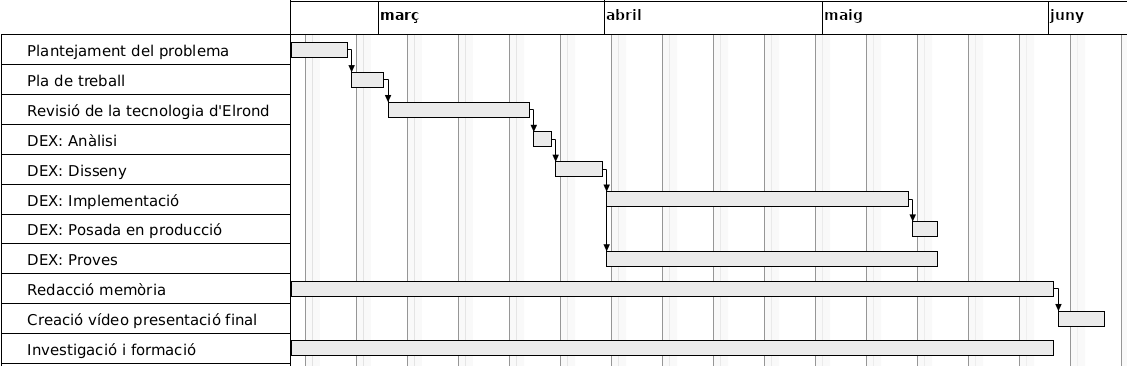
\includegraphics[width=1\textwidth]{gantt.png}
\centering
\caption{Diagrama de Gantt del projecte (creat amb GNOME Planner 0.14.6).}
\end{figure}

La següent figura presenta la temporalització de les fases del proyecte, s'ha de considerar que un dia de feina correspon a una jornada de quatre hores:
\begin{figure}[h]
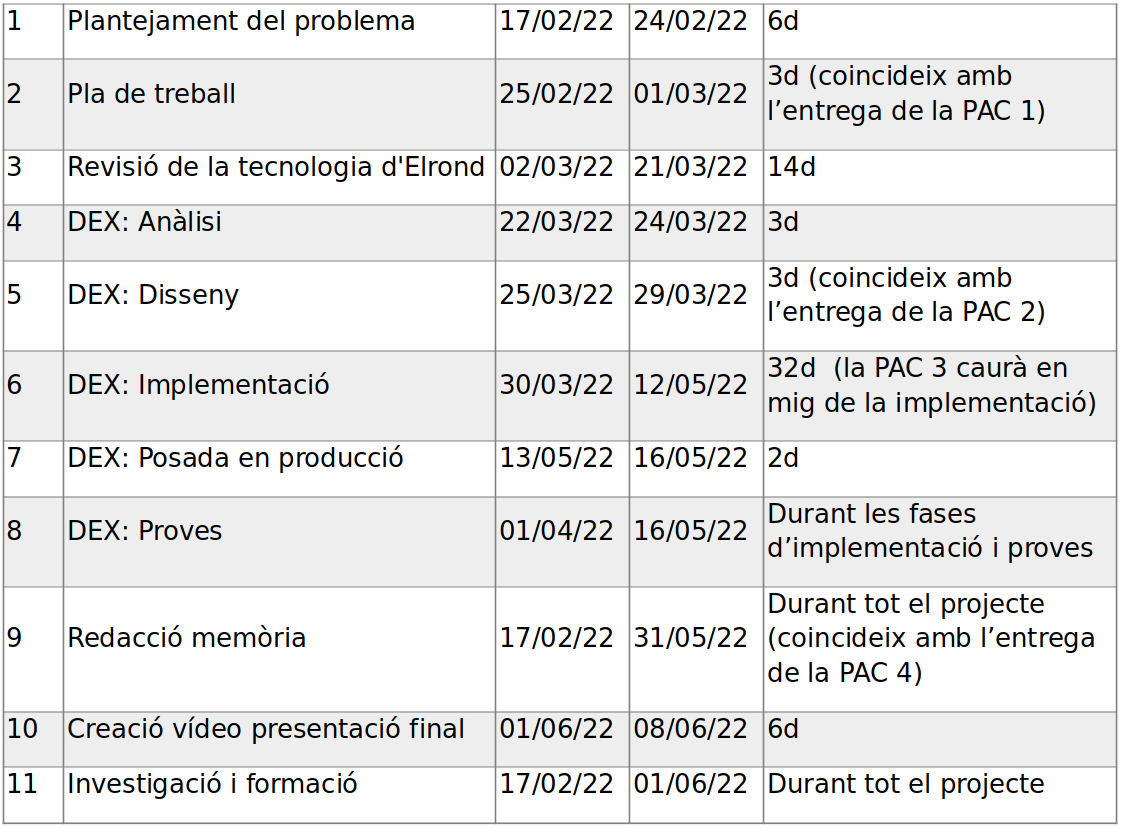
\includegraphics[width=0.85\textwidth]{gantttemp.png}
\centering
\caption{Temporalització del projecte.}
\end{figure} 

\subsection{Breu sumari de productes obtinguts}
``No hay que entrar en detalle: la descripción detallada se hará en el resto de capítulos.'' 
\medskip 

\subsection{Breu descripció dels altres capítols de la memòria}
``Explicación de los contenidos de cada capítulo y su relación con el trabajo en global.''

\newpage 

\section{Revisió de la tecnologia d'Elrond}

\subsection{Visió general de l'arquitectura}
Elrond és una cadena de blocs\footnote{En el present treball empraré indistintament ``\textit{blockchain}'' i ``cadena de blocs'' (traducció del terme proposada pel Termcat).} pública i d'alt rendiment. Altres punts a destacar són \cite{elrond2022}\cite{elrond2022-2}:
\begin{enumerate}
  \item \textbf{Entitats (usuaris i nodes)}: Els usuaris despleguen transaccions a la xarxa, en forma de transferència de valor o executant un \textit{smart contract}. Per altra banda, els nodes són dispositius en la xarxa que executen el programari d'Elrond i processen les transaccions.
  \item \textbf{\textit{Shards\footnote{No hi ha entrada al Termcat pel terme ``shard'', jo l'he traduït per ``fragment'' (empraré ambdues paraules indistintament en el present treball).}}}: Particions de la xarxa d'Elrond que permeten escalar-la. La feina de cada \textit{shard} és gestionar una part de l'estat i processar paral·lelament la corresponent part de la transacció.
  \item \textbf{\textit{Adaptive State Sharding}}: S'aplica a tots els nivells (transacció, dades i xarxa) de forma adaptativa (això és, divisió i unió dinàmica de \textit{shards} segons nombre de validadors disponibles i càrrega de la xarxa).
  \item \textbf{\textit{Validador}}: Node de la xarxa Elrond amb almenys 2500 EGLD en \textit{staking} (o bloquejats\footnote{El Termcat encara no ha traduït el terme, és una traducció pròpia que penso que fa entendre el concepte.}) que processa les transaccions i assegura la xarxa per la seva participació en el mecanisme de consens per validar els blocs (serà recompensat amb les tarifes –\textit{fees}– de les transaccions).
  \item \textbf{\textit{Secure Proof of Stake}}: Els blocs són validats per consens entre els validadors del grup de consens, que és completat en dues passes de comunicació emprant una modificació de les signatures múltiples de Boneh-Lynn-Shacham (BLS) \cite{Boneh2004}. El grup de consens és seleccionat aleatòriament i només és possible conèixer la seva composició amb una ronda d'antelaci.
  \item \textbf{Alta resiliència}: Capacitat de recuperar-se d'atacs maliciosos pel canvi de nodes entre els \textit{shards} (en cada ``època'' un terç dels nodes seran reubicats per prevenir connivències entre els mateixos).
  \item \textbf{Font d'aleatorietat segura}: Utilitzant la signatura BLS, cosa que la fa no esbiaixada i impredictible.
  \item \textbf{Elrond WASM VM}: Màquina virtual específica que permet executar contractes intel·ligents escrits en qualsevol llenguatge de programació que es permeti compilar amb  \textit{WebAssembly}\footnote{\url{https://webassembly.org/}}.
  \item \textbf{Contractes intel·ligents}: Que s'executaran emprant l'\textit{Adaptative State Sharding}. Elrond recomana que siguin escrits en Rust, però –com s'ha dit– es poden utilitzar altres llenguatges. Una característica única, comparant per exemple amb Ethereum, és que es permet modificacions dels mateixos una vedada desplegats \cite{cwirko01} (per exemple per corregir errors).
  \item \textbf{Execució ràpida de transaccions \textit{cross-shard}}: Gestionada de forma nadiua a nivell de protocol fent servir un algorisme d'expedició (\textit{dispatching}) i un algorisme d'encaminament.
   \item \textbf{\textit{Metachain}}: Cadena de blocs que s'executa en un \textit{shard} especial. El seu rol principal no és processar transaccions sinó que  és notificar i autenticar les capçaleres dels blocs processats.
   \item \textbf{Elrond Gold (EGLD)}: Criptovalor (\textit{token}) nadiu de la xarxa Elrond que serveix de mitjà de pagament per a les transaccions. Ajuda en el desplegament de dApps, en l'execució de contractes intel·ligents i també s'empra com a mecanisme de pagament pels validadors. 
\end{enumerate}

\subsection{Entitats}
\label{sub:entitat}
Bàsicament, en la xarxa Elrond hi ha dos tipus d'entitats: usuaris i nodes \cite{elrond2022}. Un \textbf{usuari} és qualsevol ens que gestioni un dels comptes –o més– de la xarxa Elrond. Això és un parell de claus criptogràfiques (una pública i una privada) que li permetran enviar transaccions signades a la xarxa. Els comptes tenen associat una quantitat d'EGLD que es coneix com a balanç i a més tenen un espai d'emmagatzematge per a valors arbitraris (com per exemple informació sobre \textit{tokens} creats pels usuaris). Els comptes s'identifiquen de forma unívoca per una adreça que coincideix amb la clau pública de l'usuari (32 bytes i fa servir la representació Bech32). Normalment, els usuaris gestionen els seus parells de claus emprant unes aplicacions informàtiques que s'anomenen carteres (o \textit{wallets})\footnote{En el present treball empraré els termes ``cartera'' o ``moneder'' indistintament per referir-me al concepte de ``\textit{wallet}''.}. Per altra banda, els \textbf{nodes} són dispositius connectats a la xarxa d'Elrond que realitzen les operacions sol·licitades pels seus usuaris. Els nodes poden ser passius (\textit{observers}) o actius (\textit{validators} i \textit{fishermen}). Els validadors s'encarreguen del consens, d'afegir blocs i mantenir l'estat, essent premiats per la seva contribució. Els \textbf{validadors} són identificats de forma única per una clau pública BLS de 96 bytes. Per garantir el correcte funcionament dels nodes, els validadors han de tenir en \textit{staking} com a mínim 2500 EGLD. Sense bloquejar EGLD els nodes poden fer d'\textbf{observadors}, però no rebran cap recompensa. Aquests darrers són membres passius de la xarxa que poden actuar com a interfície de lectura i retransmissió. Poden ser complets (\textit{full)}, mantenint tota la història de la cadena de blocs, o lleugers (\textit{light}), mantenint només 2 èpoques de l'historial de la cadena de blocs. Finalment, trobem els \textbf{pescadors} (\textit{fishermen}). La seva tasca és verificar la validesa dels blocs després d'haver estat proposats, detectant així actors maliciosos \cite{elrond2022-2}. Rebran també una recompensa i aquest rol pot ser exercit per observadors o validadors que no formin part de la ronda de consens en curs.\footnote{No es diu explícitament en la bibliografia però investigant pels grups de Telegram d'Elrond (concretament en \url{https://t.me/ElrondValidators}) vaig descobrir que el concepte de ``\textit{fisherman}'' encara no està implementat.}

\subsection{Cronologia}
En la xarxa d'Elrond s'organitza el temps en \textbf{rondes (\textit{rounds}) i èpoques (\textit{epochs})} \cite{elrond2022}. A la primera ronda de la primera època se l'anomena ronda de gènesi (\textit{genesis round}), que òbviament coincideix amb la fase d'arrencada de la xarxa.

Les \textbf{rondes} tenen una durada fixa (que actualment és configurada en 5 segons). Per l'arquitectura en \textit{shards} de la xarxa, en cada ronda només es podrà afegir un bloc a la cadena de blocs del \textit{shard}. Òbviament, si no s'arriba a consens o quan el líder del grup de consens designat és fora de línia i no pot proposar un bloc, pot haver-hi rondes en què no s'afegeixi cap bloc a la \textit{blockchain}.

Una \textbf{època} és una seqüència de rondes consecutives en què la configuració de la xarxa no canvia. El nombre de rondes en una època es calcula perquè aquesta darrera duri 24 hores (ja que aquesta és la configuració actual de la duració d'una època). Quan hi ha un canvi d'època s'aprofita per adaptar la topologia de la xarxa segons el nombre de validadors disponibles i càrrega d'aquesta, a més de per acomplir amb altres tasques per tancar l'època anterior (com calcular les recompenses per als validadors).
\medskip 

\subsection{\textit{Secure Proof of Stake}}
El funcionament \textit{Secure Proof of Stake} (SPoS) d'Elrond es pot desgranar en les següents passes \cite{elrond2022}\cite{elrond2019}: 
\begin{enumerate}
    \item La font d'aleatorietat per seleccionar els validadors per al consens es calcula a partir del bloc anterior, que és signat pel líder de consens –també conegut com a proposador de blocs o \textit{block proposer}– de la ronda que acaba. Això implica que aquesta font d'aleatorietat no podrà ser coneguda amb més d'una ronda d'antelació.
    \item Se selecciona el grup de consens, compost per validadors i un únic \textit{block proposer}. Una vegada coneguda la font d'aleatorietat, el procediment de tria del grup és determinista (triga menys de 100ms\footnote{El SPoS d'Elrond es basa en la premissa que un actor malèvol només té el temps que dura una ronda per adaptar-se i intentar influir en el bloc que es proposarà.} i no té requeriments de comunicació). S'ha de considerar que per triar els nodes es té en compte la quantitat d'EGLD en \textit{staking} i una qualificació individual –revisada al final de cada època– que es basa en el comportament passat. Per exemple, es davallarà la seva puntuació si no proposa el bloc perquè és fora de línia, es detecta una activitat maliciosa, etc. Aquesta ``meritocràcia'' anima els propietaris dels nodes a tenir-los en bon funcionament. 
    \item  El líder de consens (o validació) produeix el  bloc per a la nova ronda. Si, pel motiu que sigui, no s'ha creat un bloc en una finestra de temps s'utilitzarà la font d'aleatorietat de l'últim bloc per seleccionar un nou grup de consens.
    \item El líder de consens\footnote{Per aclarir del tot aquest punt, en la bibliografia emprada, líder de consens, líder de validació i proposador de bloc (\textit{block proposer}) fan referència al mateix concepte.} envia el bloc que acaba de proposar als validadors.
    \item  Aquests darrers components del grup validen i també signen el bloc rebut, basant-se en una modificació de \textit{Practical Byzantine Fault Tolerance} (pBFT).
    \item Els validadors trameten les signatures al \textit{block proposer}.
    \item El proposador agrega les signatures i distribueix el bloc.
    \item El \textit{hash} del bloc, la signatura, les proves d'inclusió i el nombre de \textit{shard} són tramesos a la \textit{Metachain}. 
\end{enumerate}

Aquestes passes es poden veure resumides en la Fig. \ref{fig:SPoS}.

\begin{figure}[h]
  \centering
  \begin{minipage}[b]{0.65\textwidth}
    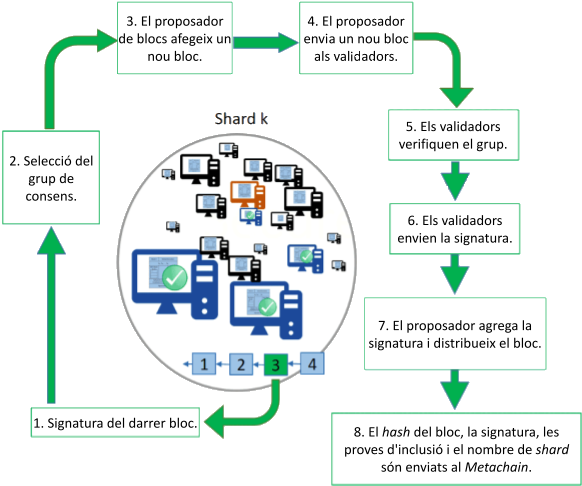
\includegraphics[width=\textwidth]{SPoS01.png}
    \caption{\textit{Secure Proof of Stake}. (Font: Modificació d'imatge dins l'apartat corresponent a SPoS a \cite{elrond2022}).}
    \label{fig:SPoS}
  \end{minipage}
  \hfill
  \begin{minipage}[b]{0.3\textwidth}
    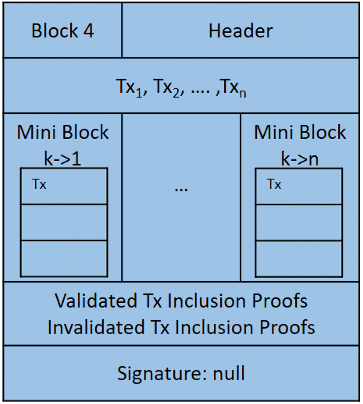
\includegraphics[width=\textwidth]{SPoS02.png}
    \caption{Estructura d'un bloc en la xarxa Elrond. (Font: Imatge dins l'apartat corresponent a SPoS a \cite{elrond2022}).}
  \end{minipage}
\end{figure}

\subsection{\textit{Adaptive State Sharding}}
El \textit{sharding} va sorgir originàriament en el camp de les bases de dades com un mètode per distribuir les dades entre múltiples màquines amb l'objectiu de suportar alt rendiment amb grans volums d'informació \cite{mongodb2021}. Elrond empra aquesta tècnica d'escalat horitzontal per particionar tant la xarxa com l'estat i processament de les transaccions amb la finalitat que diferents nodes desenvolupin la seva tasca en paral·lel (amb el consegüent augment de l'eficiència). S'ha de destacar també que s'empren els tres tipus principals de \textit{sharding} \cite{elrond2022}:

\begin{itemize}
	\item \textbf{\textit{Network sharding}}\footnote{Aquest concepte es podria traduir al català com ``fragmentació de la xarxa'' però he preferit deixar el terme anglès. El mateix passa amb \textit{transaction sharding} i \textit{state sharding}, que es podrien traduir respectivament per ``fragmentació de les transaccions'' i ``fragmentació de l'estat''.}: Gestiona com els nodes es distribueixen i agrupen entre els diferents \textit{shards}. S'ha de tenir en compte que les comunicacions dins del \textit{shard} són més ràpides que fer una propagació dels missatges a tota la xarxa (\textit{broadcast}). Però s'ha de tenir en compte que si un atacant arriba a controlar un \textit{shard} sencer suposaria un greu problema de seguretat. 
	\item \textbf{\textit{Transaction sharding}}: S'ocupa la forma en què les transaccions s'assignen als \textit{shards} encarregats del seu processament. Les transaccions són assignades a un \textit{shard} de forma determinista emprant les adreces de les transaccions.
	\item \textbf{\textit{State sharding}}: Cada \textit{shard} només manté una part de l'estat. Els dos mètodes anteriors, si no es combinessin amb aquest, haurien d'emmagatzemar una còpia sencera de tot l'estat. Així, si els comptes implicats en una transacció resideixen en \textit{shards} diferents, l'execució de la transacció implicaria l'intercanvi de missatges entre nodes per modificar els respectius estats. Per augmentar la tolerància a atacs maliciosos quan acaba una època es redistribueixen entre els diferents \textit{shards} un subconjunt dels nodes.
\end{itemize}

Com a resultat d'aquesta fusió s'aconsegueix \cite{elrond2022}:
\begin{itemize}
	\item \textbf{Escalabilitat sense afectar a la disponibilitat}: En la Fig. \ref{fig:sharding01a} podem observar la xarxa amb només un \textit{shard}. Les figures \ref{fig:sharding01b} i \ref{fig:sharding01c} mostren una arquitectura amb dos i tres \textit{shards}\footnote{En \cite{elrond2019} es pot trobar una funció en pseudocodi amb la que calcular el nombre òptim de \textit{shards}.}. Sense entrar en detall, es pot veure que augmentant o disminuint el nombre de \textit{shards} –gràcies a la forma en què s'assignen les adreces al seu fragment– s'evita temps d'inactivitat per qüestions de configuració.
	\item \textbf{Expedició (\textit{dispatching}) ràpida i traçabilitat}: La Fig. \ref{fig:sharding01c} mostra com es calcula el \textit{shard} de destí (les adreces de color blau aniran al 0, les verds a l'1 i les grogues al 2).
	\item \textbf{Eficiènia i adaptabilitat}: El sistema permet processar transaccions en paral·lel i adaptar-se a la càrrega de treball i/o estat de la xarxa. Però s'ha de destacar que la distribució dels \textit{shards} hauria de ser tan equilibrada com fos possible. Si ens fixem en la Fig. \ref{fig:sharding01c} veiem que no és equilibrada (ja que el nombre de \textit{shards} no és una potència de 2).
\end{itemize}

\begin{figure}[h]
        \centering
        \begin{subfigure}[b]{0.4\textwidth}
            \centering
            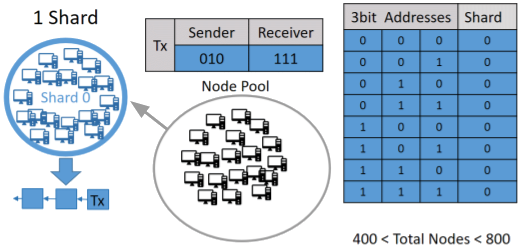
\includegraphics[width=\textwidth]{sharding01.png}
            \caption[1 \textit{shard}]%
            {{\small 1 \textit{shard}}}   
            \label{fig:sharding01a}
        \end{subfigure}
        \hfill
        \begin{subfigure}[b]{0.4\textwidth}  
            \centering 
            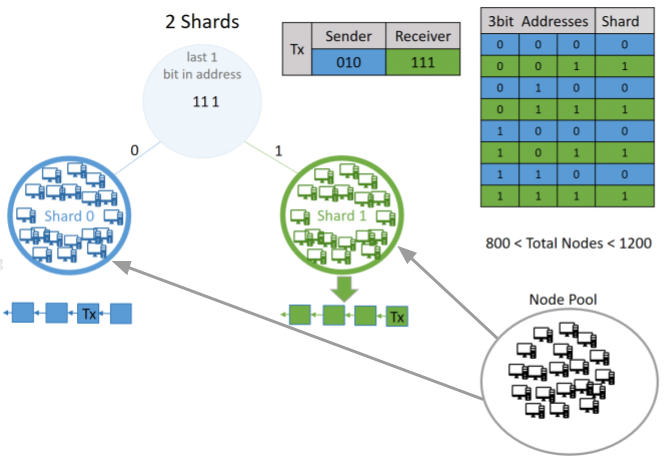
\includegraphics[width=\textwidth]{sharding02.png}
            \caption[2 \textit{shards}]%
            {{\small 2 \textit{shards}}}    
            \label{fig:sharding01b}
        \end{subfigure}
        \vskip\baselineskip
        \begin{subfigure}[b]{0.55\textwidth}   
            \centering 
            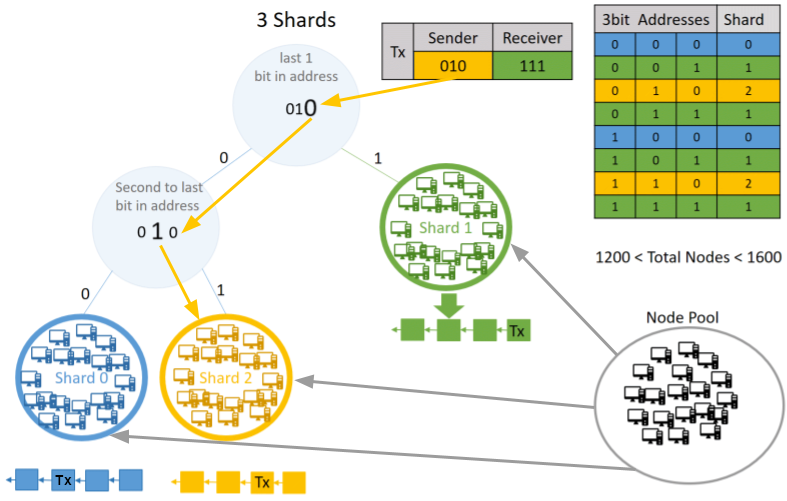
\includegraphics[width=\textwidth]{sharding03.png}
            \caption[3 \textit{shards}]%
            {{\small 3 \textit{shards}}}    
            \label{fig:sharding01c}
        \end{subfigure}
        \hfill
        \caption[La xarxa d'Elrond configurada amb un (a), dos (b) i tres (c) \textit{shards}.]
        {\small La xarxa d'Elrond configurada amb un (a), dos (b) i tres (c) \textit{shards}. (Font: Modificació d'imatge dins l'apartat \textit{Adaptive State Sharding} a \cite{elrond2022}).} 
        \label{fig:shardingtodo}
\end{figure}

Una altra cosa a destacar, referent al fraccionament de l'estat, és que els nodes guarden una \textbf{còpia de l'estat dels seus germans (redundància)} per aportar \textbf{tolerància a fallades} (Fig. \ref{fig:shardred}).

Finalment, s'ha de remarcar el fet que els \textbf{nodes es barregin entre \textit{shards} al final de cada època} per evitar la connivència entre nodes maliciosos. Això no es fa amb tots els nodes sinó que només es fa amb un nombre controlat de validadors que seran redistribuïts de manera no determinista i uniforme (aquesta tasca la realitza la \textit{metachain} emprant una font d'aleatorietat procedent del bloc anterior de la metacadena). Es fa així, i no reorganitzant tots els nodes, per maximitzar la seguretat amb la mínima introducció de latències en el sistema. Els nodes triats es col·locaran als seus nous \textit{shards} en una llista d'espera durant tota l'època actual fent la resincronització amb el nou fragment. Després el node es pot convertir en un validador elegible i unir-se al \textit{shard} efectivament.\footnote{Aquest paràgraf és un resum molt breu. Per referències més detallades consultar \cite{elrond2019}.}

\begin{figure}[h]
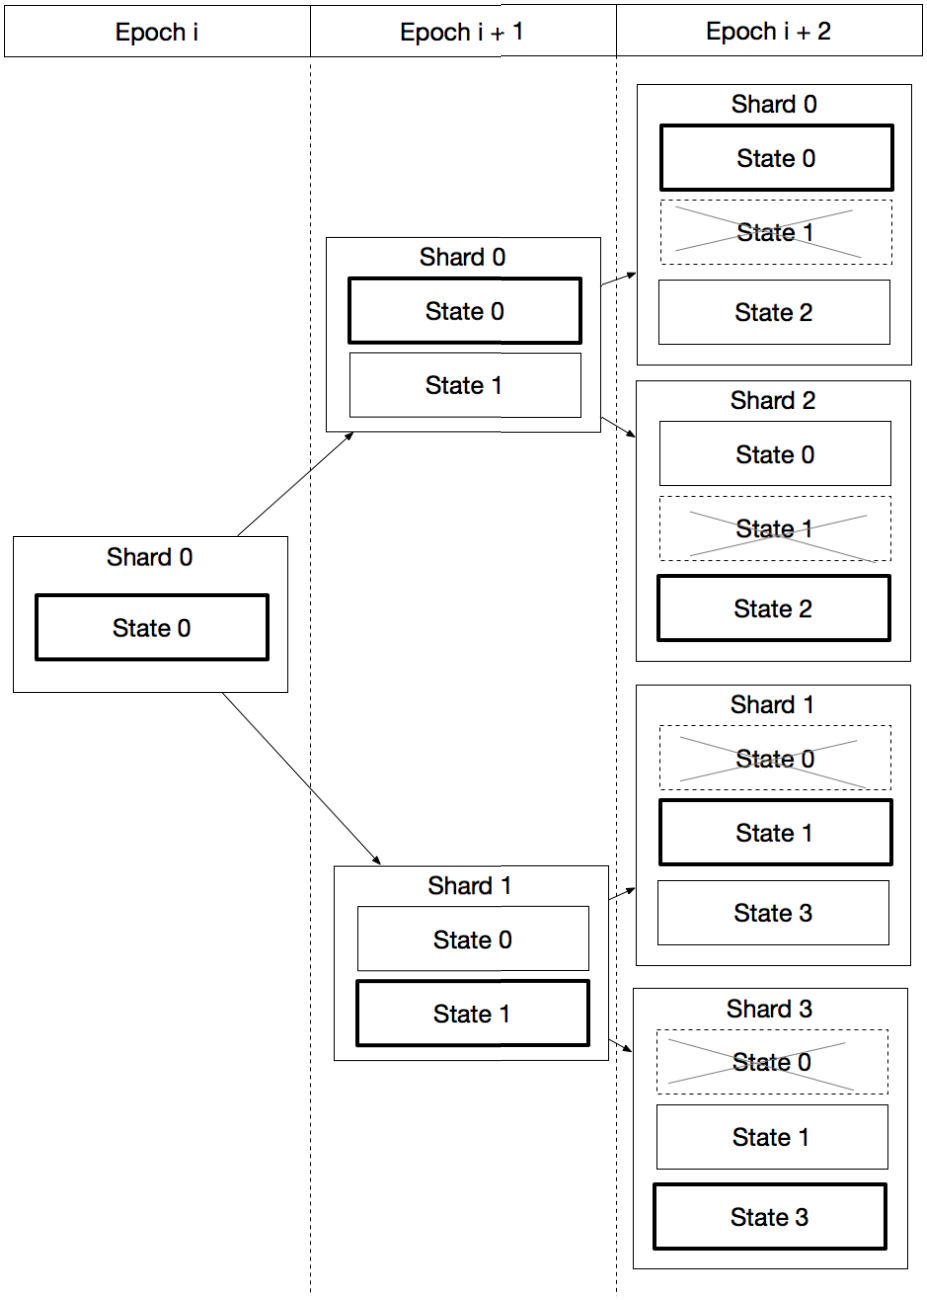
\includegraphics[width=0.4\textwidth]{shardred.png}
\centering
\caption{Redundància als \textit{shards} entre èpoques. (Font: Captura de \cite{elrond2019}).}
\label{fig:shardred}
\end{figure}

\subsection{Transaccions entre \textit{shards}}\label{sec:transshards}
Com a exemple de com s'executen les transaccions entre diferents \textit{shards} i com es comuniquen amb la \textit{metachain}, emprarem una \textbf{arquitectura amb només dos \textit{shards}}. Imaginem que un usuari des del seu \textit{wallet} amb una adreça dins del \textit{shard} 0 envia EGLD a l'adreça d'altre \textit{wallet} que es troba en el \textit{shard} 1 (Fig. \ref{fig:shardingtrans}). L'estructura dels blocs estarà formada per \cite{elrond2019}:
\begin{itemize}
	\item \textbf{Capçalera} (\textit{header}): Conté la informació referent al bloc (\textit{nonce}, \textit{round}, \textit{proposer}, \textit{validators}, \textit{timestamps}, etc.).
	\item \textbf{Llista de miniblocs}: Per a cada \textit{shard} hi haurà un minibloc que contindrà transaccions a executar. 	S'ha de destacar que un minibloc és la unitat atòmica de processament, això significa que o es processen totes les transaccions del minibloc o no es processa cap (en aquest darrer cas, es posposarà l'execució al següent \textit{round}). Dins d'un mateix bloc, poden aparèixer diversos miniblocs amb el mateix emissor i receptor (no hi ha cap limitació). Per exemple, en aquest cas simple amb només dos \textit{shards}, un bloc en el \textit{shard} 0 contindrà bàsicament tres tipus de miniblocs:
	\begin{itemize}
		\item Minibloc 0: Conté les transaccions on les adreces del remitent i del destinatari són al \textit{shard} 0. 
		\item Minibloc 1: Conté les transaccions on les adreces del remitent són al \textit{shard} 0 i les del destinatari al \textit{shard} 1.
		\item Minibloc 2: Conté les transaccions on les adreces del remitent són al \textit{shard} 1 i les del destinatari al \textit{shard} 0.
	\end{itemize}
\end{itemize}

\begin{figure}[h]
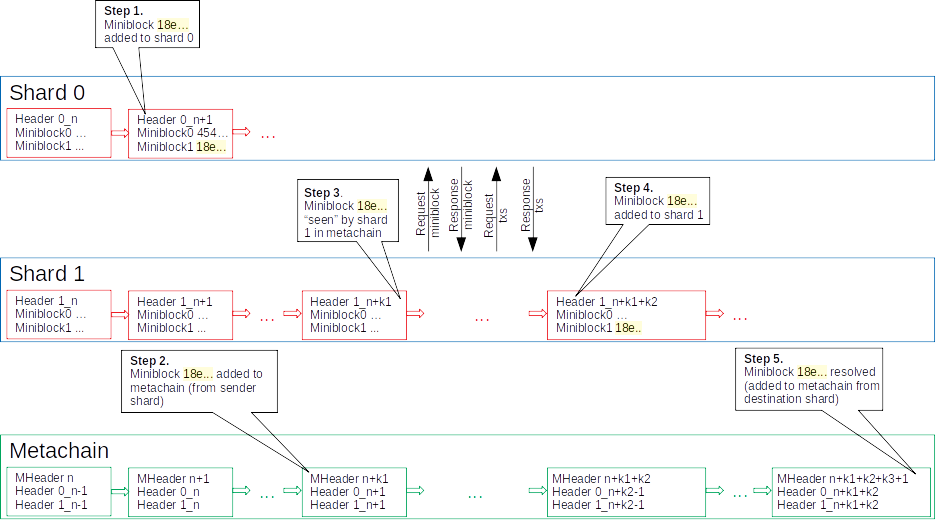
\includegraphics[width=0.9\textwidth]{shardtrans.png}
\centering
\caption{Exemple d'execució de transacció entre dos \textit{shards}. (Font: Fig. 4 de \cite{elrond2019}).}
\label{fig:shardingtrans}
\end{figure}

Observem en la \textbf{Fig. \ref{fig:shardingtrans}} un exemple de transacció asíncrona amb dos \textit{shards} implicats. Després d'arribar la transacció al \textit{shard} 0 (\textbf{\textit{step} 1}), la capçalera del bloc i els miniblocs s'envien a la \textit{metachain}. Aquesta darrera dona fe\footnote{``Donar fe'' o ``autenticar'' són les traduccions al català que he trobat més adients pel verb anglès ``to notarize''. El verb ``notarizar'' existeix en espanyol, però no existeix ``notaritzar'' en català. En qualsevol cas, empraré aquest darrer terme en algunes ocasions entre cometes per no generar confusions.} d'aquest bloc del \textit{shard} 0 creant un nou bloc a la metacadena que conté la següent informació sobre tots els miniblocs: identificador del \textit{shard} remitent, identificador del \textit{shard} receptor i \textit{hash} del minibloc (\textbf{\textit{step} 2}). El \textit{shard} 1 veu el minibloc a la \textit{metachain} i obté el seu \textit{hash} del metabloc (\textbf{\textit{step} 3}), per després demanar el minibloc al \textit{shard} 0 i executar-lo altra vegada (\textbf{\textit{step} 4}). Finalment, el \textit{shard} 1 envia el resultat a la \textit{metachain} que valida la transacció creuada (\textbf{\textit{step} 5}). En aquest punt la transacció ja es pot considerar finalitzada.

\subsection{\textit{La màquina virtual d'Elrond}}
La màquina virtual d'Elrond executa WebAssembly (Wasm)\footnote{\url{https://webassembly.org/}}, un llenguatge de baix nivell amb format binari compacte anomenat \textit{bytecode} \cite{mozilla2021}. El fet que executi Wasm implica que es puguin escriure contractes intel·ligents en qualsevol llenguatge que sigui possible compilar cap a \textit{bytecode} (C, C++, C\#, Rust, Go, TypeScript, etc.). Tot i això, Elrond recomana als desenvolupadors que emprin Rust i els hi faciliten un \textit{framework}\footnote{\url{https://github.com/ElrondNetwork/elrond-wasm-rs}} per a aquest llenguatge, així com un \textit{plugin} per a l'IDE de Microsoft Visual Studio Code\footnote{\scriptsize\url{https://marketplace.visualstudio.com/items?itemName=Elrond.vscode-elrond-ide}}. Entre les característiques a destacar de la màquina virtual d'Elrond \cite{elrond2022}\cite{mincub2020}:
\begin{itemize}
	\item \textbf{Sense estat}: Això significa que, quan un \textit{smart contract} sigui executat, es guardarà la informació en una estructura de dades transitòria, en lloc d'escriure directament en l'estat. Quan acabi l'execució, si aquesta és exitosa, l'API aplicarà els canvis a l'emmagatzematge i/o a la cadena de blocs. 
	\item \textbf{Execució fora de procés}: La màquina virtual serà executada en un procés independent i el node en si mateix en un altre, tot i que compartiran informació a través de canonades (\textit{pipes}) anònimes a memòria principal.  A més, el \textit{bytecode} s'executarà en un entorn aïllat i la memòria del procés de la màquina virtual serà inaccessible.
	\item \textbf{Motor d'execució ràpida}: Com a motor d'execució s'empra una versió modificada per Elrond de Wasmer\footnote{\url{https://wasmer.io/}}, una implementació de Wasm\footnote{Realitzada per l'empresa Wasmer Inc. que també ha creat un gestor de paquets que permet els desenvolupadors compartir mòduls empaquetats de codi Wasm.} de codi obert escrita en Rust per entorns servidor. Per les característiques de Wasmer, l'execució dels contractes intel·ligents es fa a una velocitat gairebé nadiua.
	\item \textbf{Trucades asíncrones entre contractes}: Els contractes intel·ligents poden executar trucades entre ells fent servir l'API de la màquina virtual. Com hem vist, la xarxa d'Elrond es fragmenta adaptativament, el que pot fer que es truqui a un \textit{smart contract} que es trobi en un altre \textit{shard}. En aquest cas l'execució serà asíncrona. Si ambdós estan en el mateix fragment, l'execució serà síncrona. Tot això es fa de forma transparent per al desenvolupador.
\end{itemize}

En el cas general, els contractes intel·ligents seran compilats generant un arxiu WASM que serà desplegat en alguna de les xarxes d'Elrond. 

\subsection{Execució de contractes intel·ligents en l'arquitectura amb \textit{shards}}

Un important punt a destacar és l'execució dels \textit{smart contracts} en aquesta arquitectura fragmentada. Elrond arriba a una solució amb execució asíncrona entre els \textit{shards} \cite{elrond2019}. 

El procés comença quan l'usuari crea una transacció per executar un contracte intel·ligent. Si el contracte intel·ligent no és ubicat en el mateix \textit{shard}, el cost de la transacció es lleva del compte del remitent i s'afegeix a un minibloc –segons correspongui a l'adreça del receptor– del seu \textit{shard}. La transacció és ``notaritzada'' per la \textit{metachain} i després processada pel \textit{shard} de destí. Al fragment de destí, la transacció es tracta com una invocació del mètode del contracte intel·ligent, ja que és on es troba (l'adreça de destí és la del \textit{smart contract}). Per a la trucada del contracte intel·ligent, es crea un compte temporal que suplanta el compte del remitent, amb el saldo del valor de la transacció i es crida el contracte intel·ligent. Després de l'execució, el contracte intel·ligent pot retornar resultats que afecten diversos comptes en diferents \textit{shards}. Els resultats que afecten els comptes del \textit{shard} del contracte intel·ligent s'executen a la mateixa ronda, en cas contrari es crearan transaccions \textit{Smart Contract Result} (SCR). En aquest darrer cas, es creen miniblocs SCR per a cada \textit{shard} de destí que posteriorment són ``notaritzats'' per la \textit{metachain} (de la mateixa manera que hem vist a la secció \ref{sec:transshards} per a les transaccions entre \textit{shards}). Finalment, són processats pels \textit{shards} respectius (on resideixen els comptes de destí). En el cas que un contracte intel·ligent truqui dinàmicament a un altre que es trobi en un \textit{shard} diferent, aquesta trucada es desaria com a resultat intermedi i es tractaria de la mateixa manera que per als comptes. Aquesta solució necessitarà \textbf{almenys 5 rondes per completar-se}, però té els avantatges de què \textbf{no es necessita bloqueig ni moure estats entre \textit{shards}}.

\subsection{Muntar un node validador}
Com ja s'ha deixat entreveure, la \textbf{xarxa d'Elrond} és composta pels seus nodes i per la interconnectivitat entre ells. Com s'ha dit en la secció \ref{sub:entitat}, per \textbf{node} s'entendrà qualsevol instància del programari de codi obert desenvolupat per Elrond per a aquesta tasca \footnote{Disponible a: \url{https://github.com/ElrondNetwork/elrond-go}.}. A més a més, qualsevol persona o entitat responsable de la gestió d'un o més d'aquests nodes es coneix com ``\textbf{operador de nodes}''. Com també s'ha vist, la xarxa és dissenyada per ser segura i per poder balancejar la seva càrrega. Així, quan un nou node s'uneix a la xarxa aporta més seguretat i eficiència. I la xarxa premiarà els nodes per la seva aportació, creant-se així una espècie de simbiosi.

Elrond és una xarxa descentralitzada de \textit{blockchain}, és a dir, nodes de procedència desconeguda s'uneixen per crear seqüencialment blocs amb una cadència determinada. Els blocs contenen operacions que es realitzaren a petició dels usuaris de la xarxa pagant unes taxes (\textit{fees}) per l'execució d'aquestes. Entre les operacions es troben la transferència de \textit{tokens} entre comptes o l'execució de contractes intel·ligents (totes les operacions prenen la forma de transaccions). Per tant, es defineix així un llibre de comptabilitat distribuït que no depèn de cap entitat central. 

Els nodes que estan autoritzats a prendre part en l'algorisme de consens s'anomenen \textbf{validadors}. Com que són els que veritablement produeixen i validen blocs, són els únics nodes recompensats amb EGLD per la seva contribució. Per assegurar el bon comportament dels validadors han de tenir bloquejats 2500 EGLD (\textit{stake}). Com ja vàrem dir en la secció \ref{sub:entitat}, els nodes sense \textit{stake} s'anomenen \textbf{observadors} (no participen en el consens i no guanyen recompenses). Si el validador no funciona correctament (desconnexions de la xarxa en mig del procés de consens, accions malicioses, etc.) seran ``multats'' perdent EGLD (\textit{stake slashing}) o fins i tot, en casos greus, se'ls hi llevarà l'estatus de validador (el node passarà a l'estat ``\textit{jailed}'' i no es triarà per al consens si no paga una multa de 2,5 EGLD).  Si això succeeix també davallarà la seva qualificació (\textit{rating score}). Com que aquesta puntuació defineix la fiabilitat del validador, és considerada per l'algorisme de selecció de nodes per triar el grup de consens. Així, s'afavoreix l'elecció de nodes amb qualificacions altes, també se'ls hi premiarà amb més EGLD. 

Els requeriments mínims del sistema són:
\begin{itemize}
\item 4 CPUs dedicades (Intel/AMD amb \textit{flags} SSE4.1 i SSE4.2 activats).
\item 8 GB de RAM.
\item Disc dur SSD amb 200 GB d'espai lliure.
\item Connexió a Internet de 100 Mbit/s sempre activa (mínim 4 TB/mes).
\item Sistema operatiu Linux\footnote{Es recomana Ubuntu 20.04.}/MacOS.
\end{itemize}

Com podem observar, són característiques d'un PC/Mac convencional en l'actualitat (i no d'ordinadors amb potents targetes gràfiques dedicades com passa amb el PoW de Bitcoin). No és l'objectiu del present treball, però guies com-es-fa\footnote{Traducció del Termcat del terme ``\textit{howto}''.} per instal·lar el programari per muntar un node validador en la xarxa Elrond es poden trobar a \cite{elrond2022} o \cite{penalver2019}.\footnote{Aquesta secció torna a ser una síntesi de l'apartat ``\textit{Validarors}'' de \cite{elrond2022}.}

\subsection{Xarxes Elrond disponibles}
En Elrond tenim tres xarxes disponibles:
\begin{itemize}
\item \textbf{\textit{Mainnet}}: És la xarxa en producció d'Elrond (transaccions reals amb  el pertinent cost econòmic). En el moment de redactar la present secció, té més de 3000 nodes validadors distribuïts en 3 \textit{shards} i una \textit{metachain}.
\item \textbf{\textit{Devnet}}: És una xarxa pública de proves mantinguda per la comunitat d'Elrond on qualsevol desenvolupador pot provar els seus contractes intel·ligents i dApps en un entorn real. Té uns 300 nodes validadors distribuïts en 3 \textit{shards} i una \textit{metachain}. En el present treball empraré aquesta xarxa, en detriment de \textit{testnet}, per tenir més estabilitat.
\item \textbf{\textit{Testnet}}: També pública i mantinguda per la comunitat d'Elrond, però s'empra per fer proves de futures millores i rendiment \cite{mincub2019-2} (això implica que el \textit{blockchain} es pot reiniciar\footnote{En el grup de Telegram ``\textit{Elrond Validators Announcements}'' (\url{https://t.me/ElrondValidatorsAnn}) es va definir una ronda de gènisi per la \textit{devnet} (reinici) per a dia 29 de març de 2022.}). Té uns 2000 nodes repartits en 3 \textit{shards} i un \textit{metachain}.
\end{itemize}

\begin{figure}[!htb]
\begin{subfigure}[b]{0.32\textwidth}
  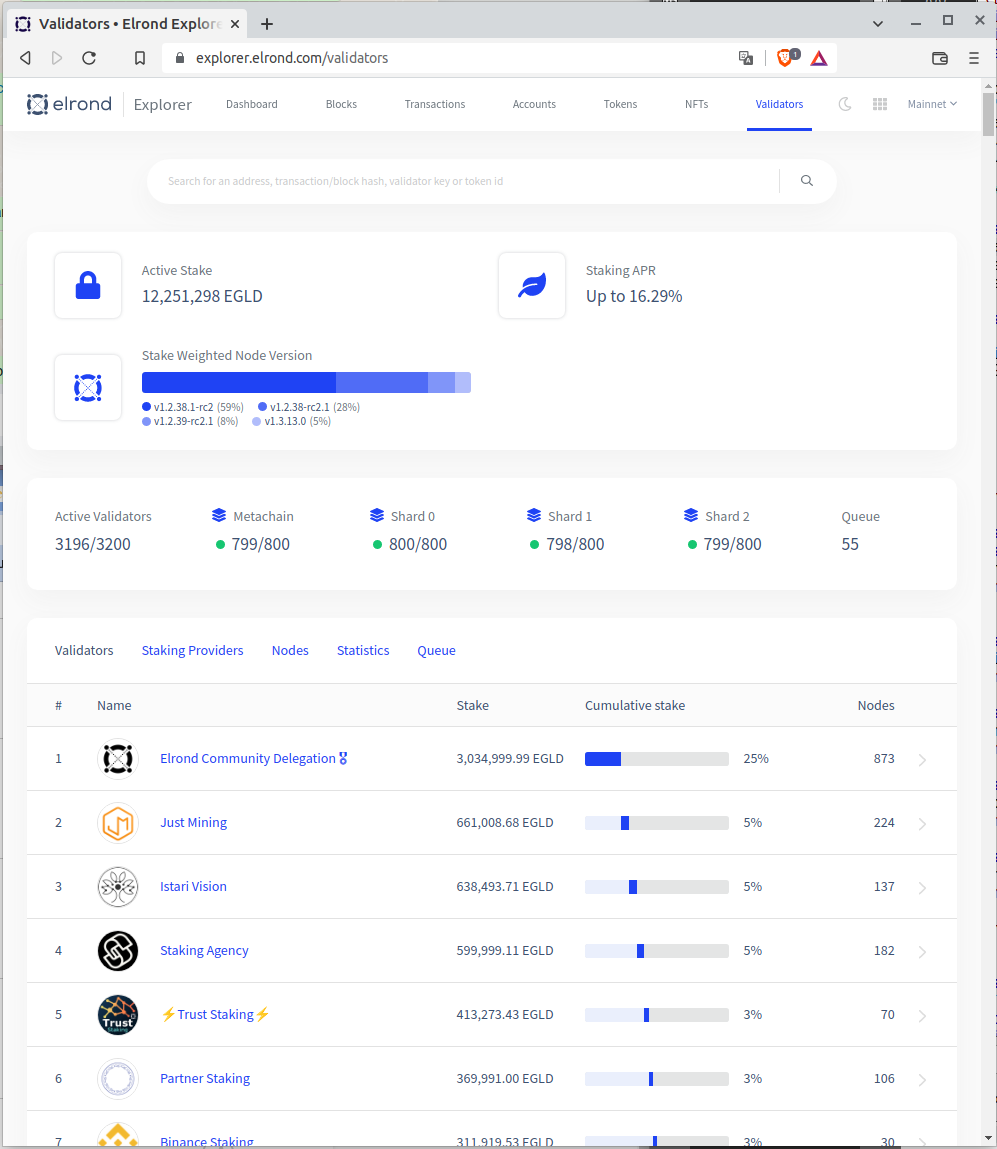
\includegraphics[width=\linewidth]{mainnet.png}
  \caption{\textit{Mainnet}: \scriptsize\url{https://explorer.elrond.com/validators}}\label{fig:mainnet}
\end{subfigure}\hfill
\begin{subfigure}[b]{0.32\textwidth}
  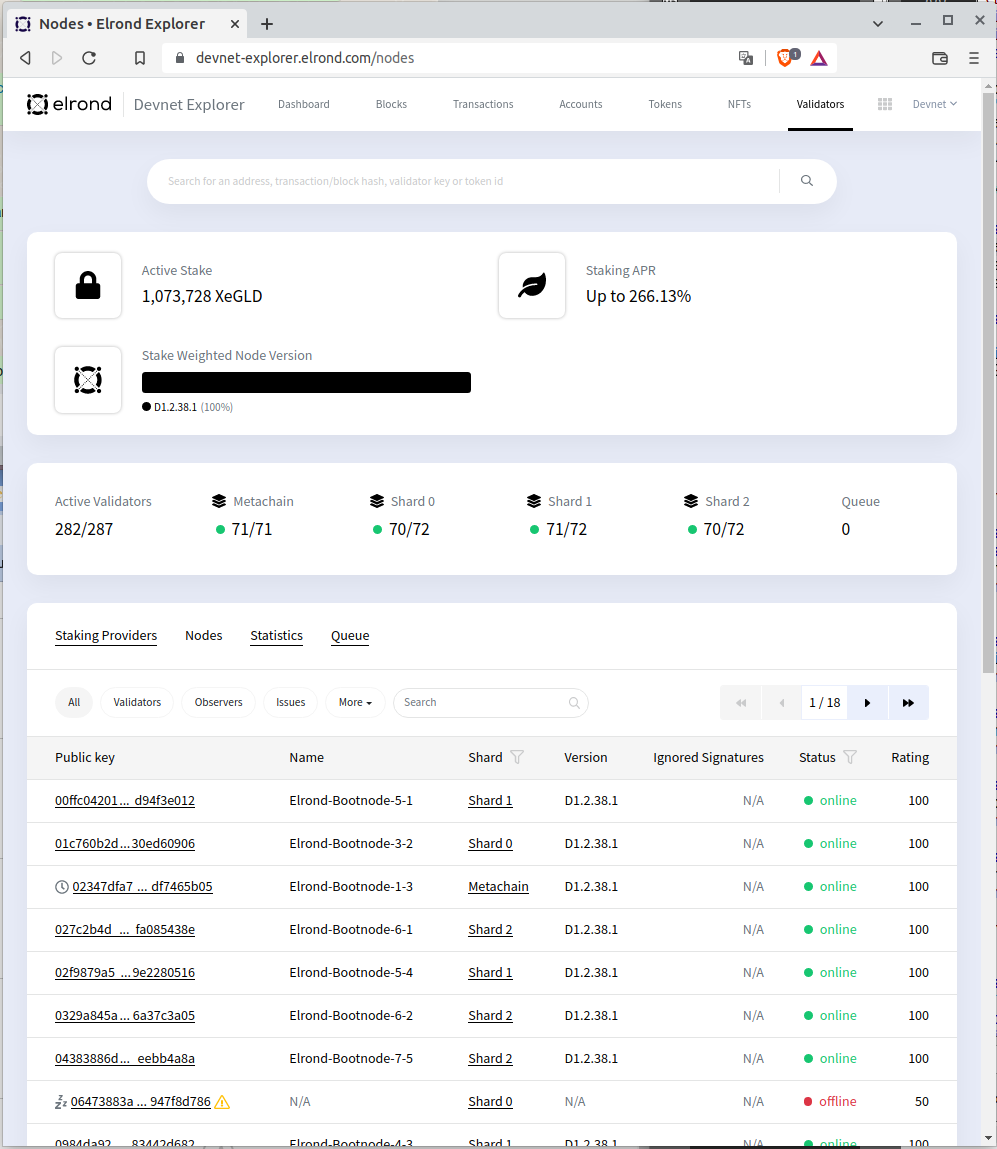
\includegraphics[width=\linewidth]{devnet.png}
  \caption{\textit{Devnet}: \scriptsize\url{https://devnet-explorer.elrond.com/nodes}}\label{fig:devnet}
\end{subfigure}\hfill
\begin{subfigure}[b]{0.32\textwidth}
  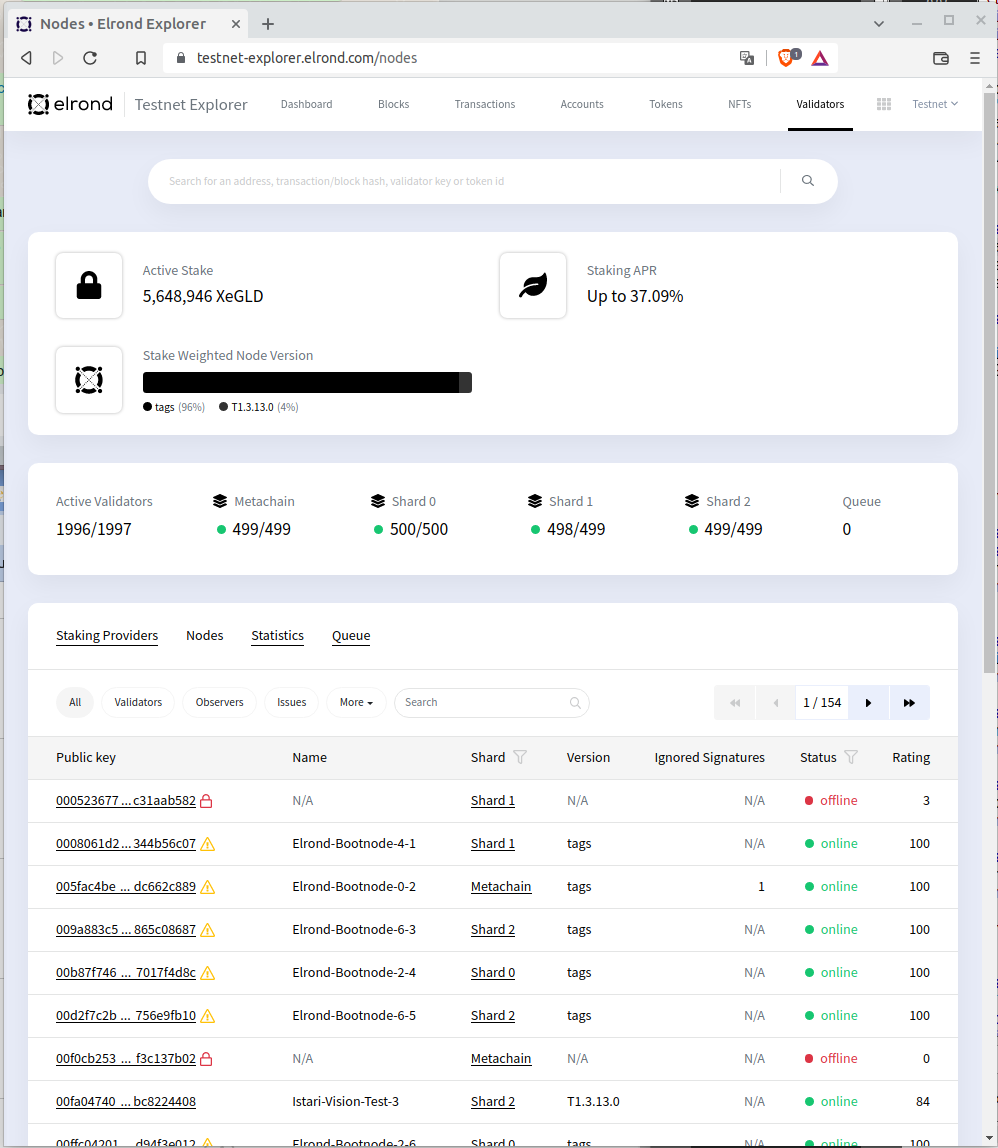
\includegraphics[width=\linewidth]{testnet.png}
  \caption{\textit{Testnet}: \scriptsize\url{https://testnet-explorer.elrond.com/nodes}}\label{fig:testnet}
\end{subfigure}\hfill
\caption{Exploradors de les xarxes disponibles a Elrond.}\label{fig:nets}
\end{figure}

\subsection{Carteres}
Com ja s'ha comentat en la secció \ref{sub:context} existeixen diferents carteres que es poden fer servir per enviar, rebre i emmagatzemar EGLD de forma segura.
\begin{itemize}
\item \textbf{Moneder web}. Existeix una versió per a cadascuna de les xarxes:\footnote{Per a la \textit{devnet} i la \textit{testnet} es disposa d'una opció \textit{Faucet} per obtenir xEGLD (que no té cap cost en moneda \textit{fiat} i et permetrà poder relalitzar transaccions).}
	\begin{itemize}
	\item \textit{Mainnet}: Accesible a \url{https://wallet.elrond.com/}.
	\item \textit{Devnet}: Accesible a \url{https://devnet-wallet.elrond.com/}.
	\item \textit{Testnet}: Accesible a \url{https://testnet-wallet.elrond.com/}.
	\end{itemize}
Tampoc és l'objectiu del present treball explicar com crear un moneder, però una guia com-es-fa es pot trobar en \cite{elrond2022}. Quan es crea s'haurà d'introduir una contrasenya\footnote{Ha de tenir almenys nou caràcters, una lletra majúscula, un símbol i un nombre.} i se'ns donaran 24 paraules secretes (que permeten generar la clau privada). El procés finalitzarà descarregant un fitxer json (\textit{keystore file}). Com es veu en la Fig. \ref{fig:webwallet}, podem accedir al nostre moneder amb aquest arxiu json i introduint la contrasenya que hem creat (1 a Fig. \ref{fig:webwallet}). Una altra opció és generar un fitxer ``PEM'' (\textit{Privacy Enhanced Mail}) amb la nostra clau privada i emprar-lo per accedir (nombre 3 a Fig. \ref{fig:webwallet}), que es pot generar emprant la utilitat d'Elrond ``erdpy'' (s'hauran d'introduir les 24 paraules secretes separades per un espai):
\begin{lstlisting}[
    basicstyle=\footnotesize,
]
erdpy --verbose wallet derive testdev-wallet.pem --mnemonic
\end{lstlisting}
Finalment, es pot iniciar sessió amb un moneder de maquinari (per exemple amb un Ledger Nano S) o llegint un codi QR amb l'aplicació mòbil Maiar (nombres 2 i 4 a Fig. \ref{fig:webwallet}, respectivament).
\begin{figure}[h]
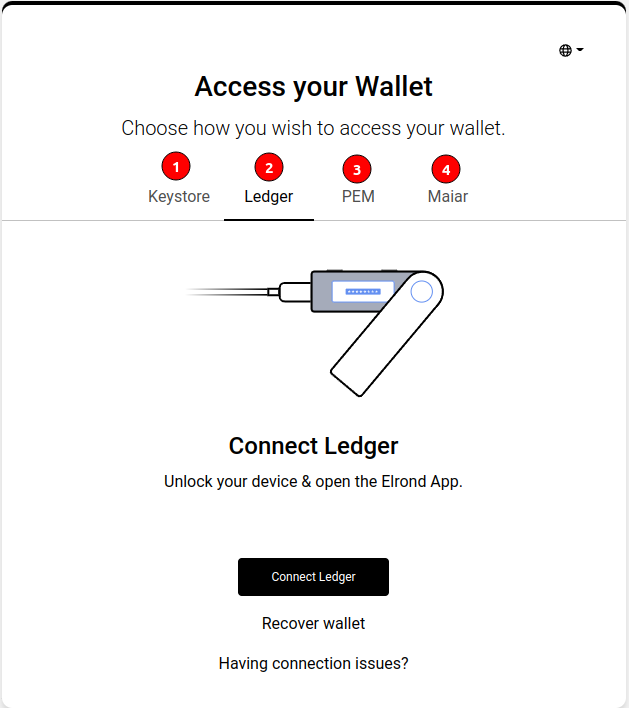
\includegraphics[width=0.5\textwidth]{webwallet.png}
\centering
\caption{Mètodes d'accés al moneder web.}\label{fig:webwallet}
\end{figure} 
\item \textbf{Maiar DeFi Wallet}. Es tracta d'una extensió per a navegadors de la família de Chrome\footnote{\url{https://chrome.google.com/webstore/detail/maiar-defi-wallet/}}. El funcionament i prestacions és similar al moneder web (i, fent la comparació, a l'extensió ``Metamask''\footnote{\url{https://metamask.io/}} de la xarxa Ethereum). En la Fig. \ref{fig:maiarwalletb} es pot observar que també es pot canviar entre les tres xarxes disponibles.
\begin{figure}[!htb]
\begin{subfigure}[b]{0.4\textwidth}
  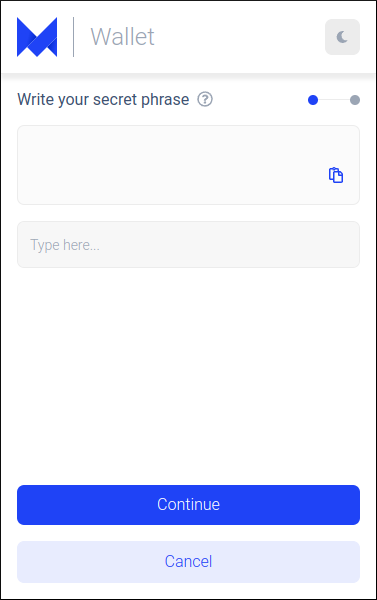
\includegraphics[width=\linewidth]{maiarextensio.png}
  \caption{}\label{fig:maiarwalleta}
\end{subfigure}\hfill
\begin{subfigure}[b]{0.4\textwidth}
  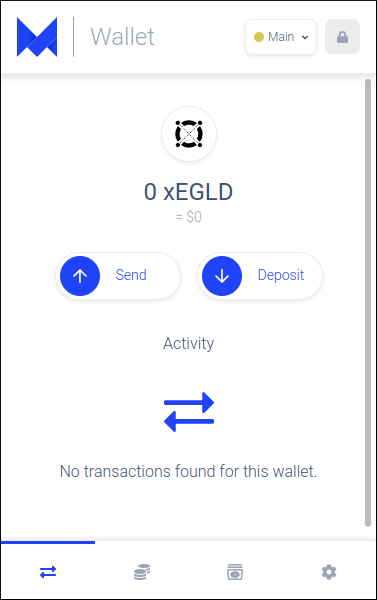
\includegraphics[width=\linewidth]{maiarextensio2.png}
  \caption{}\label{fig:maiarwalletb}
\end{subfigure}\hfill
\caption{Maiar DeFi Wallet.}\label{fig:maiarwallet}
\end{figure}
\item \textbf{\textit{Maiar}}\footnote{\url{https://maiar.com/}}. DApp que implementa una cartera digital per dispositius iOS i Android. Permet enviar o rebre diners emprant el número de telèfon mòbil o un \textit{herotag} (una espècie de nom d'usuari que es pot emprar en lloc de la teva adreça). És completament descentralitzada, sense custòdia i Elrond no té accés als fons de l'usuari en cap moment. Es pot treballar amb criptoactius com Elrond Gold (EGLD), Binance (BNB), Ethereum (ETH) o Bitcoin (BTC). Com no pot ser d'altra forma, es disposen de mecanismes de recuperació (un frase) per rescatar els fons en cas de pèrdua o robatori del nostre telèfon intel·ligent. No he trobat forma de connectar a la \textit{devnet} o \textit{testnet} des de Maiar, penso que déu ser així perquè és principalment dissenyada per treballar amb la \textit{mainnet}. Òbviament, aquesta dApp és pensada per comprar criptoactius a través de pagaments amb targeta bancària o transferències SEPA (s'han d'emprar passarel·les en ambdós casos). Curiosament, no permet fer \textit{swaps} entre criptoactius (només es poden fer des de Maiar Exchange).
\begin{figure}[h]
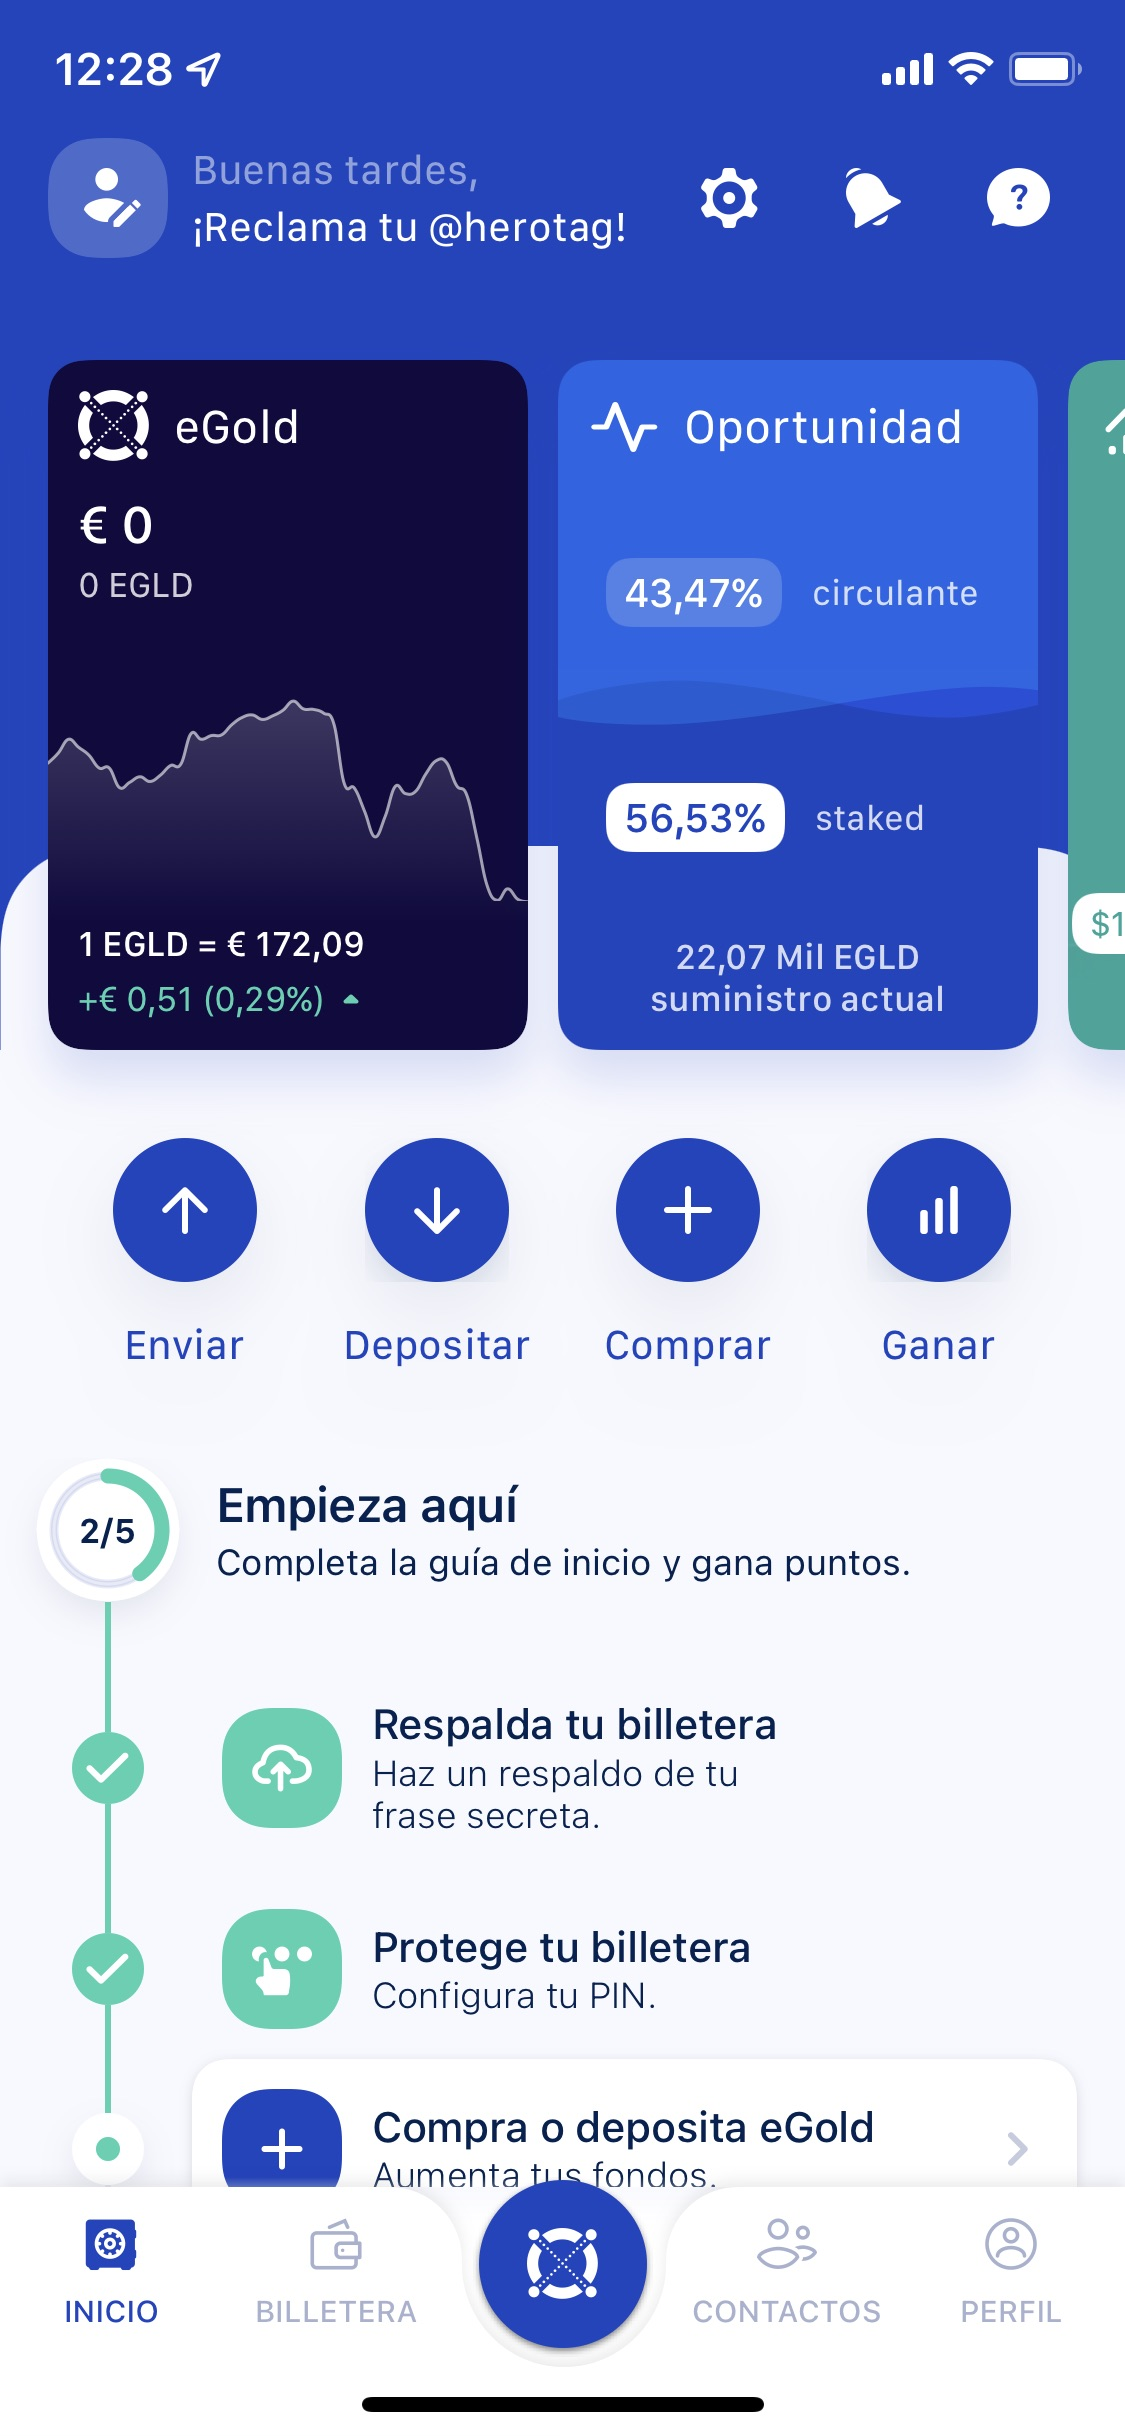
\includegraphics[width=0.3\textwidth]{maiarapp.png}
\centering
\caption{Maiar per iPhone.}\label{fig:maiarapp}
\end{figure} 
\item \textbf{\textit{Webhooks}}. Són enllaços que criden\footnote{En català balear fem ús del verb ``cridar'' en lloc del verb ``trucar''. Així diem per exemple ``cridar per telèfon'' o ``cridar el mètode d'un objecte''.} a la cartera de l'usuari perquè iniciï sessió o ompli un formulari per realitzar una transacció (del tipus pagament) amb els arguments proporcionats. Un cop realitzada l'acció, l'usuari és redirigit a un URL amb informació d'estat d'èxit o d'error. Un exemple seria \cite{elrond2022}:
\begin{lstlisting}[
    basicstyle=\scriptsize,
]
https://wallet.elrond.com/hook/login?callbackUrl=https://example.com/
\end{lstlisting}
\item \textbf{\textit{Ledger}}. Ja s'ha comentat al punt ``Moneder web'', i a més és recomanat per Elrond si es treballa amb grans quantitats d'EGLD, també podem emmagatzemar els nostres criptoactius en moneders de maquinari com són els dispositius \textit{Ledger Nano S} o \textit{Ledger Nano X}.
\end{itemize}

\subsection{Maiar Exchange}\label{subsec:maiarexchange}
Maiar Exchange\footnote{\url{https://maiar.exchange/}} és un DEX (\textit{Decentralized EXchange}) basat en \textit{liquidity pools} –fons de liquiditat– creat per Elrond emprant la seva arquitectura escalable. Permet els usuaris efectuar la compravenda de criptoactius (\textit{trading}). A més a més, els usuaris poden convertir-se en proveïdors de liquiditat aportant els seus actius (guanyant \textit{tokens} MEX per cada transacció d'intercanvi realitzada segons el parell de \textit{tokens} aportats com a reserva). MEX és el \textit{token} nadiu de Maiar Exhange. A part de tenir la funció d'incentivar els usuaris perquè proporcionin liquiditat, també s'emprarà en processos de governança. Així, ens trobem davant d'un Exchange de \textit{criptoactius} sense intermediaris, cosa que abarateix els costos de les transaccions i dels \textit{swaps}.

Entre el que podem fer amb Maiar Exchange vull destacar \cite{everstake2021}\cite{elrond2021}:
\begin{itemize}
\item \textbf{\textit{Swapping}} (intercanvi): Consisteix a intercanviar un criptoactiu per un altre. El mecanisme d'intercanvi consisteix en permutar els actius de l'usuari amb els \textit{liquidity pools} (fons de liquiditat), i no directament amb altres participants en el mercat. Els preus dels actius es fixen a partir d'una fórmula matemàtica del que s'anomena \textit{Automated Market Making}. En lloc d'utilitzar un llibre de comptabilitat com en un intercanvi tradicional, els actius tenen uns preus calculats segons un algorisme. Elrond empra la fórmula \(x * y = k\), on \(x\) és la quantitat d'un token al \textit{liquidity pool} i \(y\) és la quantitat de l'altre. \(k\) és una constant fixa, el que significa que la liquiditat total del grup sempre romandrà en la mateixa proporció. Hi ha una comissió del 0,3\% per intercanviar tokens (el 0,25\% pels proveïdors de liquiditat proporcional a la seva contribució a les reserves de liquiditat i amb la resta es compraran MEX que es cremaran). En la data de redacció d'aquesta secció, els actius entre què es poden fer intercanvis són MEX, USDC, RIDE, CRU, ZPAY, ISET, AERO, EFFORT i WAM contra  EGLD. Això significa que hi ha fons de liquiditat MEX-EGLD, EGLD-USDC, etc.
\item \textit{\textbf{Liquidity Pools}}:  Són reserves de tokens que es troben en contractes intel·ligents del DEX i estan disponibles perquè els usuaris facin intercanvis. Aquests tokens els proporcionen proveïdors de fons de liquiditat amb els quals els usuaris de la plataforma poden negociar. Els proveïdors són incentivats amb recompenses (tokens MEX) pels intercanvis que es produeixen en els seus \textit{pools} (segons s'ha explicat en el punt anterior). S'ha de destacar que els proveïdors de liquiditat en qualsevol moment poden retirar els fons que han dipositat (independentment de les condicions del mercat).  
\item \textit{\textbf{Farming}}\footnote{No m'he atrevit a traduir aquest terme, però un mot que m'agrada del català és ``conrear''.}: Consisteix en el fet que els usuaris bloquegin la seva liquiditat per obtenir recompenses. Si posem els nostres actius en un \textit{liquidity pool} obtindrem les recompenses descrites en els apartats anteriors (això és el \textit{farming} i és el que s'ha descrit en el punt d'adalt). Però hi ha també l'opció de posar els nostres \textit{liquidity pools} en \textit{staking}, el que significa que no els podrem retirar durant un temps definit a canvi d'obtenir una recompensa major.
\end{itemize}

\begin{figure}[h]
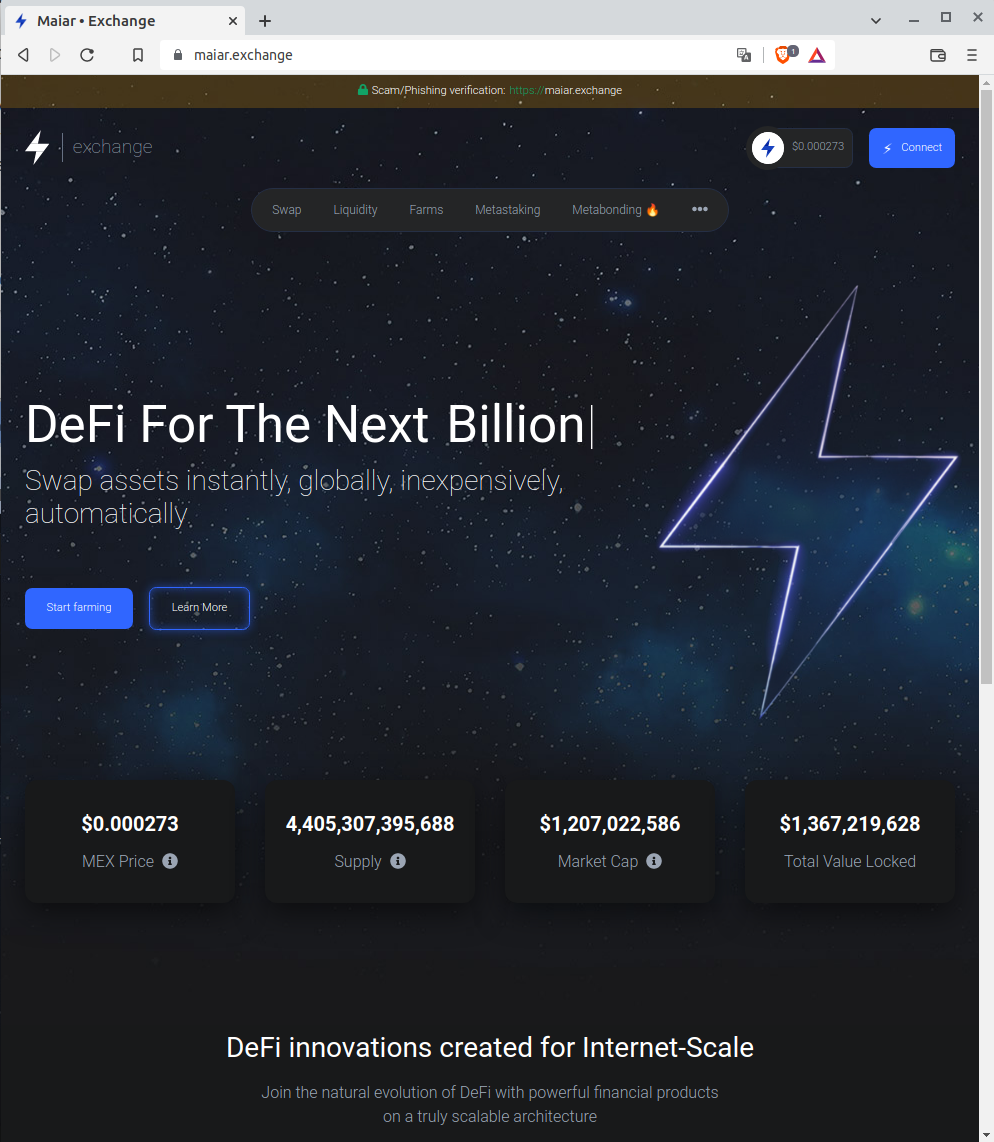
\includegraphics[width=0.75\textwidth]{maiardex.png}
\centering
\caption{Maiar Exchange.}\label{fig:maiardex}
\end{figure} 

\subsection{Altres punts destacables}\label{sub:altres}
\begin{itemize}
\item \textbf{Camps d'una transacció}:

Els camps d'una transacció sense signar en la xarxa Elrond són \cite{elrond2022}:
\begin{itemize}
\item \textbf{nonce} (\textit{number}): Nombre de seqüència del compte. És obligatori.
\item \textbf{value}	(\textit{string}): El valor a transferir. És obligatori (pot ser 0).
\item \textbf{receiver} (\textit{string}): Adreça del receptor (format \textit{bech32}). És obligatori.
\item \textbf{sender} (\textit{string}): Adreça del remitent (format \textit{bech32}). És obligatori.
\item \textbf{gasPrice} (\textit{number}): El preu del \textit{gas} que s'utilitzarà en l'abast de la transacció. És obligatori.
\item \textbf{gasLimit} (\textit{number}): El nombre màxim d'unitats de \textit{gas} assignades per a la transacció. És obligatori.
\item \textbf{data} (\textit{string}): Informació arbitrària sobre la transacció, codificada en base64 . No és obligatori.
\item \textbf{chainID} (\textit{string}): Identificador de cadena. 'D' per a la xarxa \textit{devnet}, 'T' per a \textit{textnet} i '1' per a la \textit{mainnet}. És obligatori.
\item \textbf{version} (\textit{number}): La versió de la transacció (p. ex 1). És obligatori.
\end{itemize}
En les transaccions que han de ser signades, amb la clau pública del remitent (amb l'algorisme Ed2519), s'ha d'afegir el següent camp: 
\begin{itemize}
\item \textbf{signature} (\textit{string}): Signatura digital que consta de 128 caràcters hexadecimals (64 bytes en representació en brut).
\end{itemize}
Hi ha disponibles diferents eines per realitzar la signatura des de la \textit{shell} de Linux i des del codi font: erdpy, erdwalletjs-cli o elrond-core-js.
\item \textbf{Decimals per treballar amb EGLD}: Un EGLD és configurat per tenir 18 decimals. Així, per exemple 2,5 EGLD tendrien un valor de \(2,5 * 10^{18} = 2500000000000000000\). L'usuari quan creï ESDTs podrà definir el seu nombre de decimals (amb un màxim de 18).
\item \textbf{Costos de processament} \cite{elrond2022}:
Una transacció en la xarxa Elrond té un cost de processament (\textit{processing cost}), que s'expressa com una quantitat d'unitats de \textit{gas}. Quan es llança una transacció s'ha de proporcionar un \textit{gasLimit}, que és el cost màxim que estem disposats a assumir. El \textbf{consum real de gas} (\textit{actual gas consumption} o també \textit{used gas}) és la quantitat real que s'ha consumit del \textit{gasLimit} requerida perquè la xarxa processi la transacció. Per calcular aquest darrer, la xarxa el divideix en dos components d'utilització del \textit{gas} \cite{elrond2022}:
\begin{itemize}
\item \textbf{Moviment de valors i tractament de dades}: Això seria per exemple una transferència d'EGLD entre adreces. El cost es calcula amb la fórmula:
\begin{lstlisting}[
    basicstyle=\tiny,
]
tx.gasLimit = 
    networkConfig.erd_min_gas_limit + 
    networkConfig.erd_gas_per_data_byte * lengthOf(tx.data)
Nota:
networkConfig.erd_min_gas_limit <= tx.gasLimit i
tx.gasLimit <= networkConfig.erd_max_gas_per_transaction
\end{lstlisting}
\item \textbf{Execució de contracte intel·ligent}: Una trucada a un \textit{smart contract} requeriria aquest i l'anterior. El cost és més difícil de determinar, ja que depèn del codi font concret del contracte intel·ligent. Es solen emprar simulacions i estimacions.
\end{itemize}
Finalment, la \textbf{tarifa de processament} (\textit{processing fee}) es calcula amb respecte de l'\textit{actual gas consumption} i dels seus dos components. Per moviment de valors i tractament de dades s'especifica en la transacció un \textit{gas price per gas unit} (que ha de ser igual o superior al paràmetre de la xarxa \(erdmin\textunderscore  gas\textunderscore price\)). Per execució de contracte intel·ligent el \textit{gas price per gas unit} es calcula respecte a un altre paràmetre de xarxa anomenat \(erd\textunderscore gas\textunderscore price\textunderscore modifier\):
\begin{lstlisting}[
    basicstyle=\tiny,
]
value_movement_and_data_handling_price_per_unit = tx.GasPrice
contract_execution_price_per_unit = tx.GasPrice * networkConfig.erd_gas_price_modifier
\end{lstlisting}

\item \textbf{ESDT (\textit{Elrond Standard Digital Token})}: La xarxa Elrond admet de forma nadiua l'emissió de \textit{tokens} creats pels usuaris (des de codi, des d'un contracte intel·ligent o des de la \textit{web wallet}). Això implica que no és necessari emprar contractes com els de tipus ERC20 de la xarxa Ethereum. Ja que el suport és nadiu, no es requereix processament extra per part de la màquina virtual (amb el que són tan eficients com el mateix EGLD).

\item \textbf{NFT (\textit{Non-Fungible Token}) i SFT (\textit{Semi-Fungible Token})}: Suport nadiu d'NFT i SFT afegint metadades i atributs a sobre de l'ESDT. Així, són bastant similars a aquests darrers però amb atributs extra (\textit{NFT Name}, \textit{Quantity}, \textit{Royalties}, \textit{Hash}, \textit{Attributes} i \textit{URI}).

\item \textbf{\textit{Local Testnet}}: Es pot configurar una \textit{testnet} en local per fer proves i \textit{debugging} del codi. Es pot configurar amb l'eina \textit{erdpy} i conté nodes validadors, nodes observadors, un \textit{seed node} i un \textit{Elrond Proxy}.

\item  \textbf{API REST}: Té dues capes a les quals es pot accedir públicament:
\begin{itemize}
\item \textbf{https://gateway.elrond.com}: La de més baix nivell. Gestiona l'encaminament de les peticions de forma transparent segons els mecanismes de fragmentació que s'han descrit en els apartats anteriors.
\item \textbf{https://api.elrond.com}:  La de més alt nivell (empra els serveis de la capa anterior). Aporta serveis com un mecanisme de memòria cau, cerques històriques amb Elasticsearch\footnote{\url{https://www.elastic.co/}}, etc.
\end{itemize}
\end{itemize}

\newpage 

\section{testDEX}

\subsection{Anàlisi}
\subsubsection{DEX i AMM}

Un \textbf{\textit{Decentralized exchange} (DEX)} és un mercat on els negociants de criptomonedes fan transaccions directament entre ells –d'igual a igual (\textit{peer-to-peer})– sense haver de lliurar la gestió dels seus fons a un intermediari \cite{cointelegraph}. És a dir, són dissenyats per eliminar qualsevol autoritat de supervisió en els intercanvis (\textit{swaps}) de criptoactius, evitant que s'hagin d'enviar dades de caràcter personal (noms, adreces, etc.). Per executar les ordres d'intercanvi sense intermediaris s'empren contractes intel·ligents. Això xoca amb el concepte de \textit{\textbf{Centralized exchange}} on la gestió és responsabilitat d'una organització, com ara un banc o qualsevol altra corporació, que requerirà que els seus usuaris estiguin identificats i que custodiaran els actius dels usuaris (òbviament cercant un benefici econòmic).
 
En el present treball ens centrarem en una versió simplificada de DEX fent servir \textit{Automated Market Makers} (AMM). Els diferents tipus de DEX es poden observar en la figura \ref{fig:dextypes}.
\begin{figure}[h]
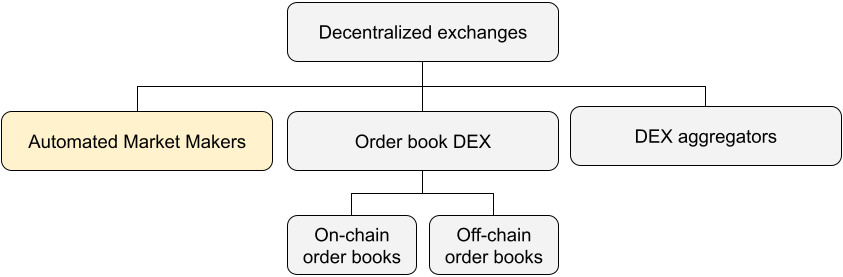
\includegraphics[width=0.95\textwidth]{DEXtypes.png}
\centering
\caption{Tipus de DEX. (Font: \cite{cointelegraph}).}\label{fig:dextypes}
\end{figure} 

En \cite{delarosa} es descriu que una de les formes de prescindir del llibre d'ordres d'un \textit{Exchange} tradicional és emprant AMM. Aquests protocols fan servir una fórmula matemàtica per calcular el preu de l'actiu i un fons de liquiditat per a cada parell de criptoactius (tal qual hem vist en la secció \ref{subsec:maiarexchange}). Quan es vulgui fer un intercanvi entre criptoactius s'interactuarà directament amb un contracte intel·ligent que determinarà el preu de compra de l'actiu destí segons l'estat del fons de liquiditat. La fórmula per calcular això, també vista en la secció \ref{subsec:maiarexchange}, és  \(x * y = k\) (amb \(x\) la quantitat d'un token al fons de liquiditat, \(y\) és la quantitat de l'altre i \(k\) és una constant fixa per mantenir la proporcionalitat entre el parell de \textit{tokens}). Així, imaginem que tenim un fons de liquiditat amb el parell xEGLD-UOC –``UOC'' és un ESDT creat per mi– amb 10 xEGLD i 100000000 UOC. Tenint que \(x * y = k\) i, pel fons descrit, la fórmula quedarà com a \(10 * 100000000 = 1000000000\). Si volem calcular la quantitat \(q_{withoutFee}\) d'UOC que obtindríem per 1 xEGLD en aquest fons:

$$ (10 + 1) * (100000000 - q_{withoutFee}) = 1000000000 $$
$$ 1100000000 - 11 * q_{withoutFee} = 1000000000 $$
$$ 1100000000 - 1000000000 = 11 * q_{withoutFee} $$
$$ 100000000 = 11 * q_{withoutFee} $$
$$ q_{withoutFee} = 100000000 / 11 $$
$$ q_{withoutFee} = 9090909,090909091 $$

A partir del resultat anterior, podem calcular el \textbf{la quantitat d'UOC que obtindrem amb 1 EGLD}:
$$ price_{EGLD-UOC} = q_{withoutFee} / q_{EGLD} $$
$$ price_{EGLD-UOC} = 9090909,090909091 / 1 = 9090909,090909091 $$

Ara tenim que el \textit{liquidity pool} ha quedat amb el parell xEGLD-UOC com \(11-90909090,909090909\) (\(90909090,909090909=100000000-9090909,090909091\)). Amb això tenim que \(11 * 90909090,909090909 = 1000000000 \) (es manté la constant \(k\))\footnote{Aquesta operació deixa intuir que per mantenir el valor de \(k\) constant serà un problema, ja que l'arrodoniment provocarà que s'acumuli error.}. El \textbf{preu pagat per una unitat d'UOC en EGLD} haurà estat:
$$ price_{UOC-EGLD} = 1 / 9090909,090909091 = 0,00000011 $$

En el procediment anterior no hem aplicat cap comissió, i com s'ha dit els \textit{liquity providers} aportaran als fons de liquiditat parells d'actius obtenint una recompensa segons els \textit{swaps} que es realitzin amb els seus parells. Recalculant la fórmula d'abans aplicant una comissió \(fee_{EGLD}\):
$$ (10 + (1 - fee_{EGLD})) * (100000000 - q_{withFee}) = 1000000000 $$
$$ 11 - 10 * fee_{EGLD}) * (100000000 - q_{withFee}) = 1000000000 $$
$$ 11 * (100000000 - q_{withFee}) - 10 * fee_{EGLD} * (100000000 - q_{withFee}) = 1000000000 $$
$$ 1100000000 - 11 * q_{withFee} - 1000000000 * fee_{EGLD} + 10 * fee_{EGLD} * q_{withFee} = 1000000000 $$
$$ -11 * q_{withFee} + 10 * fee_{EGLD} * q_{withFee} = 1000000000 - 1100000000 + 1000000000 * fee_{EGLD} $$
$$ q_{withFee} * (-11 + 10 * fee_{EGLD}) = -100000000 + 1000000000 * fee_{EGLD} $$
$$ q_{withFee} = (-100000000 + 1000000000 * fee_{EGLD}) / (-11 + 10 * fee_{EGLD}) $$

Aplicant, per exemple, una comissió del 0,3\%:
$$ q_{withFee} = (-100000000 + 1000000000 * 0,003) / (-11 + 10 * 0,003) $$
$$ q_{withFee} = -97000000 / -10,97 $$
$$ q_{withFee} = 8842297,174111212 $$

I el \textbf{preu en EGLD per unitat d'UOC} haurà estat (augmenta un poc per la comissió):
$$ price_{UOC-EGLD} = 1 / 8842297,174111212 = 0,000000113 $$

També podem calcular a partir de la fórmula anterior la \textbf{comissió pagada en EGLD} (\(fee_{EGLD}\)):
$$ q_{withFee} * (-11 + 10 * fee_{EGLD}) = -100000000 + 1000000000 * fee_{EGLD} $$
$$ -11 * q_{withFee} + 11 * 10 * fee_{EGLD} = -100000000 + 1000000000 * fee_{EGLD} $$
$$ 11 * 10 * fee_{EGLD} - 1000000000 * fee_{EGLD} = -100000000 + 11 * q_{withFee} $$
$$ fee_{EGLD} * (11 * 10 - 1000000000) = -100000000 + 11 * q_{withFee} $$
$$ fee_{EGLD}= (-100000000 + 11 * q_{withFee}) / (11 * 10 - 1000000000) $$

Com que ja hem calculat \(q_{withFee}\):
$$ fee_{EGLD} = (-100000000 + 11 * 8842297,174111212) / (11 * 10 - 1000000000) $$
$$ fee_{EGLD} = -2734731,084776668 / -999999890 $$
$$ fee_{EGLD} = 0,002734731 $$

Finalment, podem calcular la \textbf{comissió en UOC} (\(fee_{UOC}\)) fent la substracció de quantitat d'UOC que es dona sense i amb comissió:
$$ fee_{UOC} = q_{withoutFee} - q_{withFee} $$
$$ fee_{UOC} = 9090909,090909091 - 8842297,174111212 $$
$$ fee_{UOC} = 248611,916797879 $$

Si tornem a comprovar la constant \(k\), tenim que el \textit{liquidity pool} ha quedat amb el parell xEGLD-UOC com \(10 + 1 \) i \(100000000 - 8842297,1741112121 - 248611,916797879\) (s'ha de pensar que la comissió s'ha de llevar del pool perquè se li envia al proveïdor de liquiditat). És a dir, \(11\) i \(90909090,909090909\). Amb això tenim que \(11 * 90909090,909090909 = 1000000000 \). Així, l'usuari haurà pagat \(1\) xEGLD per \(9090909,090909091\) UOC i el fons de liquiditat mantindrà la mateixa constant \(k\). El \textbf{preu pagat per una unitat de UOC en EGLD} haurà estat:
$$ price_{UOC-EGLD} = 1 / 9090909,090909091 = 0,00000011 $$

En resum, amb aquest exemple s'ha mostrat que amb 1 xEGLD l'usuari ha pagat 0,002734731 xEGLD de comissió i ha rebut 8842297,174111212 UOC. La citada comissió serà tramesa al moneder del proveïdor de liquiditat automàticament.

A tot això se li ha d'afegir una cosa més: \textbf{la comissió que pagarà l'usuari a la xarxa Elrond}. En la secció \ref{sub:altres} s'ha vist que emprar la xarxa Elrond duu associat uns costos pel moviment de valors i tractament de dades (transferim una quantitat de tokens al contracte intel·ligent) i per execució de contracte intel·ligent (el \textit{smart contract} que implementa l'AMM). Això encarirà l'operació a l'usuari i les operacions que es realitzen dins aquest contracte influiran en el cost. En temps de disseny s'haurà de triar una opció òptima a nivell de repercusió en els costos de l'usuari.

\subsubsection{Les variants de DEX i AMM a testDEX}
Per assolir els objectius del projecte no fa falta arribar a desenvolupar un DEX de l'estil de Maiar Exchange, Uniswap\footnote{\url{https://uniswap.org/}} o PancakeSwap\footnote{\url{https://pancakeswap.finance/}}. Òbviament, un projecte d'aquesta envergagura seria poc realista per una limitació clara de temps. Per exemple, el protocol AMM no és exempt de problemes que s'haurien de tractar \cite{vuterin2018}. Així en aquesta versió inicial faré una sèrie d'adaptacions per ajustar-me al temps disponible:
\begin{itemize}
\item El propietari del contracte intel·ligent serà l'únic que pot definir \textit{liquidity pools}.
\item El propietari del contracte serà, per tant, l'únic que rebi les comissions pels \textit{swaps}.
\item Tots els parells tindran com a un dels seus components EGLD.
\end{itemize}

\subsubsection{Requeriments funcionals}\label{subsub:rfun}
Els requeriments funcionals responen a la pregunta ``què ha de fer un sistema''. Pel present projecte s'especifiquen els següents:
\begin{itemize}
\item RF 1: El sistema permetrà el propietari del contracte intel·ligent dipositar un parell EGLD-ESDT en el fons de liquiditat des del seu \textit{wallet}.
\item RF 2: El sistema permetrà el propietari del contracte intel·ligent recuperar un parell EGLD-ESDT del fons de liquiditat cap al seu \textit{wallet}, que prèviament haurà dipositat.
\item RF 3: El sistema permetrà el propietari del contracte definir una taxa (``\textit{fee}'') que serà gravada als usuaris quan intercanviïn \textit{tokens}.
\item RF 4: El sistema permetrà el propietari recuperar els guanys acumulats al seu contracte intel·ligent resultant del pagament de l'anterior taxa cap al seu \textit{wallet}.
\item RF 5: El sistema permetrà els usuaris intercanviar (\textit{swap}) una quantitat d'un \textit{token} ESDT de la cartera de l'usuari per un altre del fons de liquiditat (si existeix el parell adient).
\item RF 6: El sistema permetrà els usuaris conèixer els parells donats d'alta al DEX.
\item RF 7: El sistema permetrà els usuaris consultar si un parell és disponible per fer \textit{swaps} (cap dels dos components pot tenir valor 0).
\item RF 8: El sistema permetrà els usuaris consultar la constant K d'un parell en un moment donat.
\item RF 9: El sistema mostrarà els preus dels actius en el moment actual (tant de compra com de venda).
\item RF 10: El sistema enregistrarà el resultat de les transaccions per realitzar estadístiques.
\end{itemize}

\subsubsection{Requeriments no funcionals}\label{subsub:rnofun}
Els requeriments no funcionals responen a la pregunta ``com ha de fer un sistema''. Pel present projecte s'especifiquen els següents:
\begin{itemize}
\item RNF 1: La informació emprada en el sistema viatjarà per la xarxa emprant protocols segurs.
\item RNF 2: El sistema serà accessible des de qualsevol ubicació a través d'Internet.
\item RNF 3: Els usuaris del sistema el podran emprar utilitzant qualsevol moneder vàlid de la xarxa Elrond.
\end{itemize}

\subsection{Disseny}

\subsubsection{Casos d'ús}

Tindrem un usuari privilegiat (el propietari del contracte intel·ligent) i usuaris genèrics. El primer, òbviament, podrà realitzar també les operacions dels segons. El sistema permetrà només el propietari interactuar amb el contracte intel·ligent de la següent forma:{\footnote{He imitat els diagrames explicatius de la documentació d'Elrond \cite{elrond2022} i per això no he fet servir diagrames de casos d'ús d'UML. El contingut de les figures es troba en anglès ja que és l'idioma que he emprat en el codi font.}}

\begin{figure}[!htb]
\begin{subfigure}[b]{0.485\textwidth}
  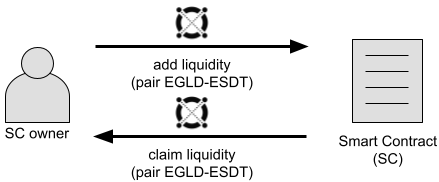
\includegraphics[width=\linewidth]{cu_add_claim_liquidity.png}
  \caption{Requerimens funcionals 1 i 2.}\label{fig:addclaimliq}
\end{subfigure}\hfill
\begin{subfigure}[b]{0.49\textwidth}
  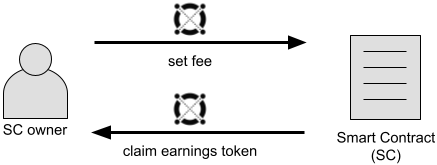
\includegraphics[width=\linewidth]{cu_set_fee_claim_earnings.png}
  \caption{Requeriments funcionals 3 i 4.}\label{fig:setfeeclaim}
\end{subfigure}\hfill
\caption{Interaccions del propietari amb el contracte intel·ligent.}
\end{figure}

Amb les interaccions anteriors es podran \textbf{definir \textit{liquity pools}} i una \textbf{taxa (\textit{fee})} que es cobrarà per les operacions de \textit{swap}. Allò següent a definir seran els intercanvis en si mateixos. El criptoactiu de referència serà EGLD (tots els parells el tindran). Així es podrà passar una determinada quantitat d'EGLD a una quantitat d'ESDT, això també es pot anomenar ``\textbf{comprar ESDT amb EGLD}''. A la inversa, podrem passar ESDT a EGLD, que dit d'altra forma seria ``\textbf{vendre ESDT per EGLD}''. La següent figura ho mostra:
\begin{figure}[!htb]
\begin{subfigure}[b]{0.49\textwidth}
  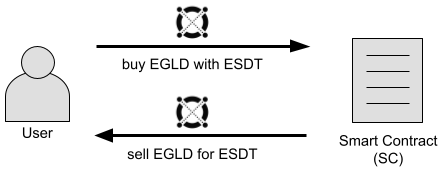
\includegraphics[width=\linewidth]{cu_buy_sell2.png}
  \caption{RF 5 (EGLD-ESDT).}\label{fig:buysell1}
\end{subfigure}\hfill
\begin{subfigure}[b]{0.49\textwidth}
  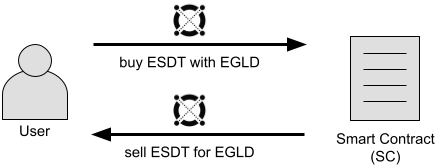
\includegraphics[width=\linewidth]{cu_buy_sell1.png}
  \caption{RF 5 (ESDT-EGLD).}\label{fig:buysell2}
\end{subfigure}\hfill
\caption{Operacions de compra i venda de \textit{tokens} (\textit{swaps}).}
\end{figure}

Per altra banda, serà necessari que el sistema mostri als usuaris els \textbf{parells disponibles per fer intercanvis i si es pot operar amb ells en un moment donat} (requeriments funcionals 6 i 7).

\begin{figure}[!htb]
\begin{subfigure}[b]{0.49\textwidth}
  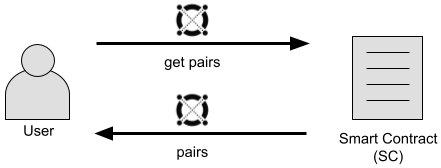
\includegraphics[width=\linewidth]{cu_get_pairs.png}
  \caption{RF 6.}\label{fig:statuspair}
\end{subfigure}\hfill
\begin{subfigure}[b]{0.49\textwidth}
  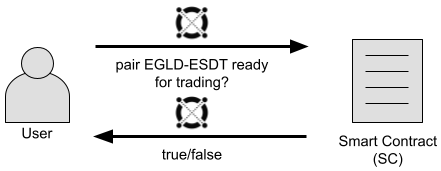
\includegraphics[width=\linewidth]{cu_status_pair.png}
  \caption{RF 7.}\label{fig:statuspair}
\end{subfigure}\hfill
\caption{Parells donats d'alta preparats per a intercanvis.}
\end{figure}

A més, el sistema mostrarà la \textbf{constant \(k\) del protocol AMM} (que s'ha de mantenir constant) i el \textbf{preu dels actius en el moment actual}. Internament es treballa amb nombres sencers on es destinen les 18 posicions a la dreta per decimals, però realment són nombres sencers. Això farà que la constant \(k\) pugui fluctuar i que estigui sotmesa a correccions per mantenir-la en el seu valor inicial. Així mateix, els usuaris hauran de conèixer en temps real els preus de les parelles de tokens. Els casos d'ús sobre aquests punts es mostren en la Fig. \ref{fig:RRFF8-9}.

\begin{figure}[!htb]
\begin{subfigure}[b]{0.33\textwidth}
  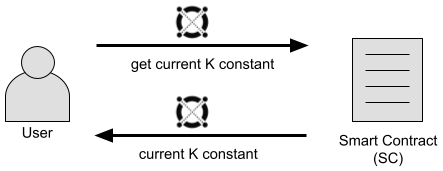
\includegraphics[width=\linewidth]{cu_k_constant.png}
  \caption{RF 8.}\label{fig:statuspair}
\end{subfigure}\hfill
\begin{subfigure}[b]{0.33\textwidth}
  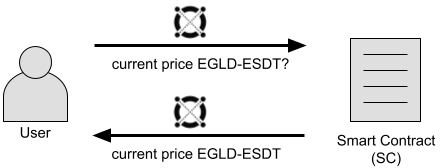
\includegraphics[width=\linewidth]{cu_current_price_EGLD_ESDT.png}
  \caption{RF 9 (EGLD-ESDT).}\label{fig:price_egld_esdt}
\end{subfigure}\hfill
\begin{subfigure}[b]{0.33\textwidth}
  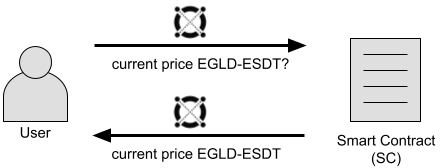
\includegraphics[width=\linewidth]{cu_current_price_EGLD_ESDT.png}
  \caption{RF 9 (ESDT-EGLD).}\label{fig:price_egld_esdt}
\end{subfigure}\hfill
\caption{Valor actual de la constant \(k\) i preus de compra-venda dels parells de \textit{tokens}.}
\label{fig:RRFF8-9}
\end{figure}

El darrer requeriment funcional és un poc especial i fa referència a què \textbf{el sistema tractarà el resultat de les transaccions} per generar estadístiques per intentar comprovar les característiques de la xarxa Elrond.

\begin{figure}[h]
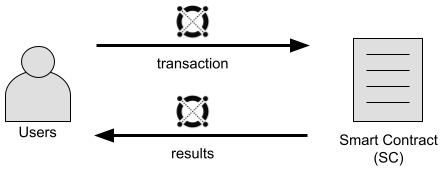
\includegraphics[width=0.55\textwidth]{cu_trans_results.png}
\centering
\caption{Requeriment funcional 10.}\label{fig:transresults}
\end{figure} 

Finalment, pel que fa als \textbf{requeriments no funcionals}, no cal afegir res ja que formen part de les característiques intrínseques de les tecnologies d'Internet i de la xarxa Elrond.

\subsubsection{\textit{Smart contract}}
El contracte intel·ligent serà públic a la xarxa \textit{devnet} d'Elrond. S'ha de remarcar que totes les dades dels \textit{smart contracts} són disponibles públicament, tot i que pot ser complicat cercar manualment l'emmagatzematge del contracte i per això es solen definir \textit{getters} públics\footnote{Quan s'implementin les propietats i mètodes públics en el lleguatge Rust s'anotaran amb \#[endpoint] o \#[view].}. Quan es desplegui a la xarxa se li assignarà automàticament una adreça amb el format que s'ha descrit en seccions anteriors.

En la Fig. \ref{fig:testdex} es mostren les propietats i mètodes del contracte intel·ligent que emprarem (anomenat ``TestDEX''). Cal dir, que en argot específic de \textit{blockchain} seria més apropiat anomenar a una propietat ``emmagatzematge''. 

\begin{figure}[h]
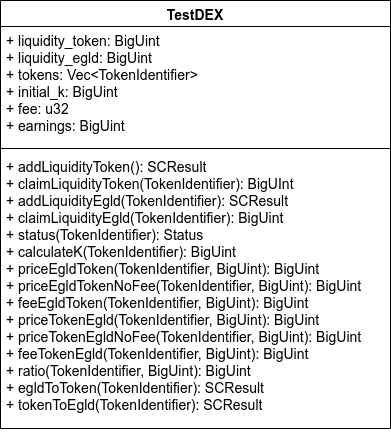
\includegraphics[width=0.55\textwidth]{TestDEX.png}
\centering
\caption{Estructura del contracte intel·ligent.}\label{fig:testdex}
\end{figure} 

Aquesta és la seva descripció:
\begin{itemize}
\item \textbf{liquidity\_token(TokenIdentifier)}: Emmagatzema la liquiditat dels \textit{tokens} (la meitat del parell). Per als identificadors del token dels que volguem guardar la informació, tindrem un valor del tipus BigUint\footnote{Estructura de dades que representa un nombre sencer molt gran sense signe.} associat que defineix la quantitat de \textit{token}.
\item \textbf{liquidity\_egld(TokenIdentifier)}: Guarda la liquiditat en EGLD dels \textit{token} (l'altra part del parell). Per als identificadors del token dels que volguem guardar la informació, tindrem un valor del tipus BigUint associat que defineix la quantitat d'EGLD.
\item \textbf{tokens}: Guarda un vector de TokenIdentifier, que descriu els \textit{tokens} dels que disposem un parell disponible –\textit{token}-EGLD o EGLD-\textit{token}– per operar.
\item \textbf{initial\_k(TokenIdentifier)}: Per a cada parell (EGLD o EGLD-\textit{token}), emmagatzema un BigUint amb la seva constant \(k\) del moment en què es va donar d'alta. 
\item \textbf{fee}: Guarda la taxa –amb un valor del tipus u32\footnote{Sencer sense signe representat amb 32 bits.}– que s'aplicarà quan es faci un intercanvi. S'inicialitza quan es creï el contracte intel·ligent.
\item \textbf{earnings\_egld(TokenIdentifier)}: Emmagatzema les taxes (\textit{fees}) –BigUint– cobrades pels diferents \textit{tokens}.
\item \textbf{init(u32)}: Mètode que realitza la tasca de constructor del contracte intel·ligent. Se li passa la taxa que es cobrarà en els intercanvis.
\item \textbf{add\_liquidity\_token() -\textgreater SCResult}: Afegeix liquiditat a la part ``\textit{token}'' del parell. Retorna un \(enum\) anomenat SCResult, forma predeterminada de retornar opcionalment un error (\(Err(SCError)\)) o una confirmació de resultat satisfactori (\(Ok(T)\)). El token i la quantitat les agafarà de la mateixa transacció dins de la xarxa Elrond. Mètode que només pot ser cridat pel propietari del contracte.
\item \textbf{claim\_liquidity\_token(TokenIdentifier)  -\textgreater SCResult}: Envia els fons de liquiditat d'un \textit{token} determinat aportats pel propietari del contracte intel·ligent a l'adreça del seu moneder. Se li ha de passar com a paràmetre l'identificador del \textit{token} del qual volem reclamar la liquiditat. Mètode que només pot ser cridat pel propietari del contracte. Retorna un BigUint equivalent a la quantitat transferida. El parell quedarà en estat ``Funding''.
\item \textbf{add\_liquidity\_egld(TokenIdentifier)  -\textgreater SCResult}: Afegeix liquiditat a la part EGLD del parell. Se li ha de passar com a paràmetre l'identificador d'EGLD. La quantitat l'agafarà de la mateixa transacció dins de la xarxa Elrond. Mètode que només pot ser cridat pel propietari del contracte.
\item \textbf{claim\_liquidity\_egld(TokenIdentifier)  -\textgreater SCResult}: Envia els fons de liquiditat en EGLD del parell d'un determinat \textit{token} aportats pel propietari del contracte intel·ligent a l'adreça del seu moneder. Se li ha de passar com a paràmetre l'identificador del token del que volem guardar la informació. Mètode que només pot ser cridat pel propietari del contracte. Retorna un BigUint equivalent a la quantitat transferida. El parell quedarà en estat ``Funding''.
\item \textbf{status(TokenIdentifier) -\textgreater Status}: Mostra l'estat d'un parell. Tindrà dos possibles estats: ``Successful'' i ``Funding''. El primer significa que està preparat per fer intercanvis i el segon indica que encara s'han d'afegir fons a algun dels components del parell. Se li ha de passar com a paràmetre l'identificador del \textit{token} del que volem retornar aquesta informació. Retorna o bé ``Successful'' o bé ``Funding''.
\item \textbf{calculate\_k(TokenIdentifier) -\textgreater BigUint}: Calcula la constant \(k\) per a un parell en un moment donat de temps. Se li ha de passar com a paràmetre l'identificador del token que identifica el parell del que volem retornar aquesta informació (el que no sigui EGLD). Retorna la citada constant.
\item \textbf{claim\_earnings(TokenIdentifier) -\textgreater BigUint}: Envia els beneficis acumulats al contracte resultants d'aplicar la taxa als intercanvis d'un \textit{token} determinat. Se li ha de passar com a paràmetre l'identificador del \textit{token} del que volem transferir els beneficis. Mètode que només pot ser cridat pel propietari del contracte. Retorna un BigUint equivalent a la quantitat transferida.
\item \textbf{price\_egld\_token(TokenIdentifier, BigUint) -\textgreater BigUint}: Calcula el preu d'una certa quantitat d'un \textit{token} determinat en EGLD. Se li ha de passar com a arguments l'identificador del \textit{token} del que volen calcular el preu i la citada quantitat. Retorna el preu com a nombre sencer. S'aplica la taxa (\textit{fee}).
\item \textbf{price\_egld\_token\_no\_fee(TokenIdentifier, BigUint)-\textgreater BigUint}: Igual que l'anterior però al preu retornat no se li aplica la taxa.
\item \textbf{fee\_egld\_token(TokenIdentifier, BigUint) -\textgreater BigUint}:  Calcula la taxa que es pagarà per una certa quantitat d'un \textit{token} determinat en EGLD. Se li ha de passar com a arguments l'identificador del \textit{token} del que volen calcular el preu i la citada quantitat. Retorna aquest cost com a nombre sencer.
\item \textbf{price\_token\_egld(TokenIdentifier, BigUint) -\textgreater BigUint}: Calcula el preu d'una certa quantitat d'EGLD en un \textit{token} determinat. Se li ha de passar com a arguments l'identificador del \textit{token} amb el que volem pagar i la quantitat d'EGLD que volem obtenir. Retorna el preu com a nombre sencer. S'aplica la taxa (\textit{fee}).
\item \textbf{price\_token\_egld\_no\_fee(TokenIdentifier, BigUint) -\textgreater BigUint}: Igual que l'anterior però al preu retornat no se li aplica la taxa.
\item \textbf{fee\_token\_egld(TokenIdentifier, BigUint) -\textgreater BigUint}: Calcula la taxa que es pagarà per una certa quantitat d'EGLD en un \textit{token} determinat. Se li ha de passar com a arguments l'identificador del \textit{token} i la citada quantitat. Retorna aquest cost com a nombre sencer.
\item \textbf{ratio(TokenIdentifier) -\textgreater BigUint}: Retorna un nombre sencer amb la relació que hi ha entre els \textit{tokens} que formen el parell. Si la relació és 0 perquè el primer és més petit que l'altre, es retornarà 1. S'emprarà per corregir la constant \(k\) per evitar l'error introduit pel redondeig de nombres sencers. Se li ha de passar com a argument el \textit{token} que identifica el parell.
\item \textbf{egld\_to\_token(TokenIdentifier) -\textgreater SCResult}: Compra de \textit{token} amb EGLD. La quantitat d'EGLD s'agafarà de la transacció. S'enviarà la quantitat del \textit{token} al moneder de l'usuari que faci la compra. Les taxes pagades s'acumularan al contracte intel·ligent. S'haurà de passar com a argument l'identificador del \textit{token} que es vol comprar. Les taxes es llevaran de la quantitat que ha de rebre l'usuari com a resultat de l'intercanvi
\item \textbf{token\_to\_egld() -\textgreater SCResult}: Compra d'EGLD amb \textit{token}. El \textit{token} i la quantitat d'EGLD s'agafaran de la transacció. S'enviarà la quantitat d'EGLD al moneder de l'usuari que faci la compra. Les taxes pagades s'acumularan al contracte intel·ligent. Les taxes es llevaran de la quantitat que ha de rebre l'usuari com a resultat de l'intercanvi.
\end{itemize}
 
\subsubsection{Arquitectura}

Una \textbf{dApp} ens permetrà escriure en la blockchain i llegir l'emmagatzematge –o estat– del contracte intel·ligent descrit en l'apartat anterior. Com es pot comprovar en la Fig. \ref{fig:architecture} \textbf{per escriure en la cadena de blocs} la dApp haurà de llençar una \textbf{transacció} que invoqui a un mètode del contracte. Si per contra només necessitem \textbf{llegir l'estat} del contracte intel·ligent, emprarem una \textbf{API} aportada per Elrond per invocar certs mètodes del contracte, cosa que no farà pas cap canvi en la cadena de blocs.

\begin{figure}[h]
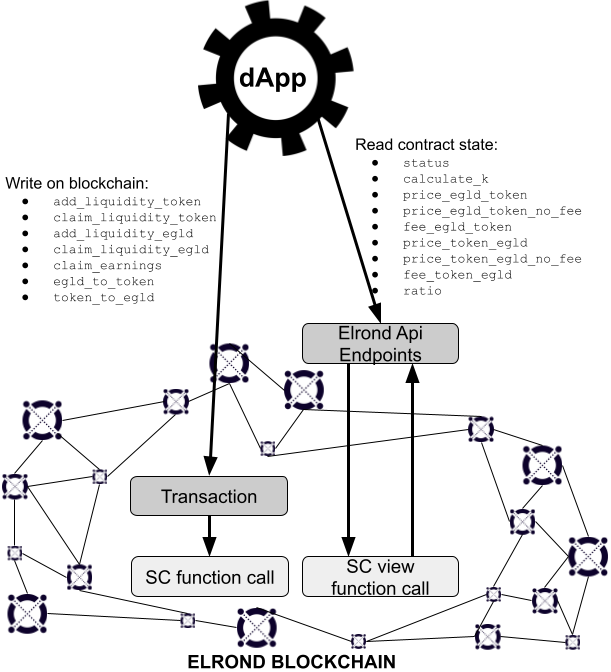
\includegraphics[width=0.75\textwidth]{architecture.png}
\centering
\caption{Arquitectura de testDEX. (Font: Elaboració pròpia inspirada en \cite{elrond2022}).}\label{fig:architecture}
\end{figure} 

Pot parèixer una descripció molt breu, però és que és veritablement una arquitectura molt senzilla.

\subsubsection{Pantalles}

Per \textbf{accedir a la dApp} s'haurà de triar un dels mètodes habilitats per fer-ho a la xarxa Elrond (Fig. \ref{fig:screen_login}).

\begin{figure}[h]
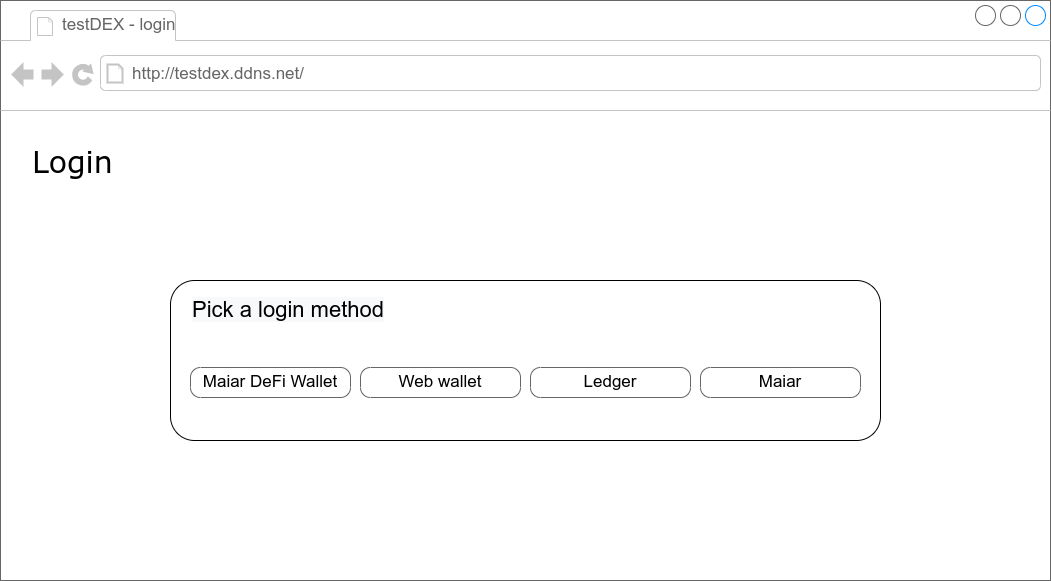
\includegraphics[width=0.9\textwidth]{screen_login.png}
\centering
\caption{Finestra de login.}\label{fig:screen_login}
\end{figure} 

Només per a l'\textbf{usuari que sigui el propietari del contracte}, li apareixerà en el menú d'adalt a la dreta l'\textbf{opció ``Fund''}. En aquesta pantalla podrà \textbf{crear els diferents fons de liquidesa del contracte intel·ligent} (Fig. \ref{fig:screen_fund}).

\begin{figure}[h]
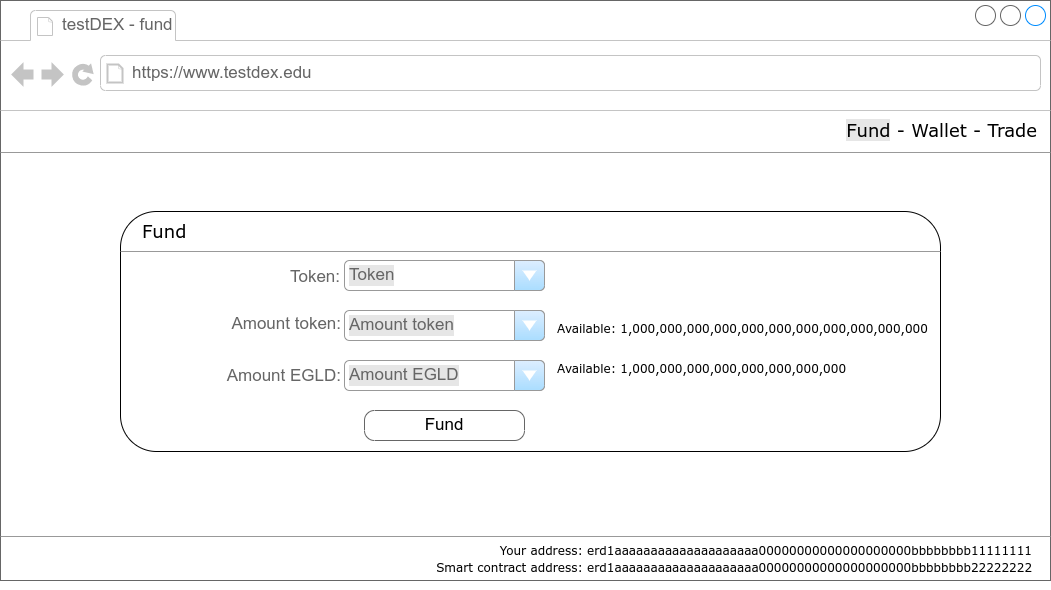
\includegraphics[width=0.9\textwidth]{screen_fund.png}
\centering
\caption{Finestra on es provisionen els \textit{liquidity pools}.}\label{fig:screen_fund}
\end{figure} 

L'\textbf{opció de menú ``Wallet''} simplement ens durà a una finestra on l'usuari podrà comprovar l'\textbf{estat del seu moneder} (Fig. \ref{fig:screen_wallet}).

\begin{figure}[h]
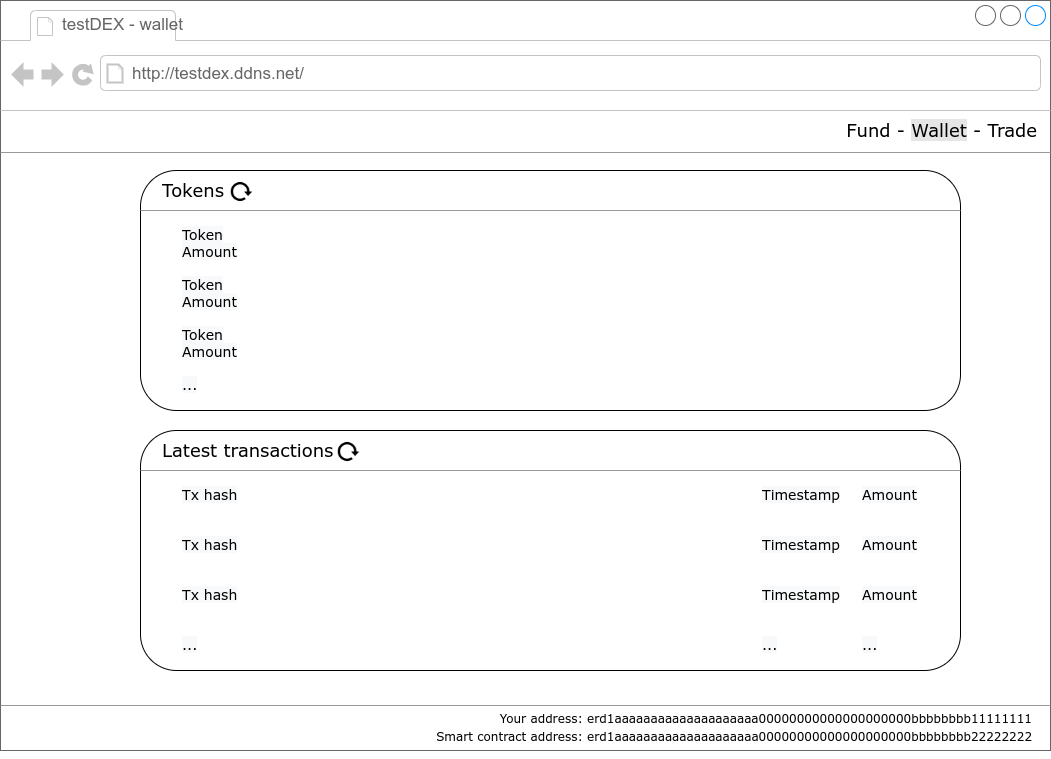
\includegraphics[width=0.9\textwidth]{screen_wallet.png}
\centering
\caption{Finestra on es mostra el moneder de l'usuari.}\label{fig:screen_wallet}
\end{figure} 

En l'\textbf{opció del menú ``Trade''} trobem la finestra amb el cor de l'aplicació (Fig. \ref{fig:screen_trade}). Podem observar que apareixerà un gràfic on es pot consultar l'\textbf{evolució dels preus del parell en el temps}. A la dreta del gràfic es podran \textbf{seleccionar el parells i realitzar compres o vendes}. En la part inferior de la pantalla, a l'esquerra apareixerà un \textbf{històric de les operacions fetes} i a la seva dreta les \textbf{estadístiques sobre les transaccions}. \textbf{Es mesuraran el nombre de transaccions, el temps transcorregut i la mitjana de transaccions per minut}.

\begin{figure}[h]
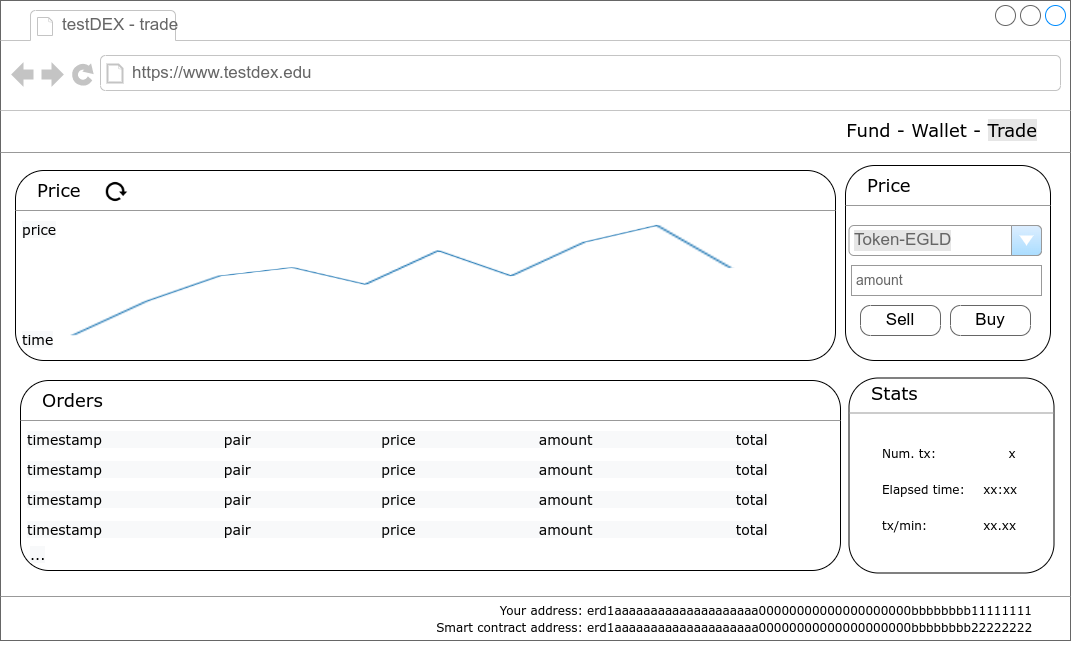
\includegraphics[width=0.9\textwidth]{screen_trade.png}
\centering
\caption{Finestra on es fan els intercanvis.}\label{fig:screen_trade}
\end{figure} 


\subsection{Implementació}

\subsection{Posada en producció}
Començarem compilant el contracte intel·ligent. Executarem dins el directori on es trobi el codi font del contracte intel·ligent:
\begin{lstlisting}[
    basicstyle=\footnotesize,
]
erdpy contract build
\end{lstlisting}

Amb això generarem el fitxer ``testdex.wasm'' que desplegarem a la \textit{devnet} d'Elrond amb la comanda:
\begin{lstlisting}[
    basicstyle=\footnotesize,
]
erdpy contract deploy --pem="~/wallet/wallet1.pem" \
  --recall-nonce --gas-limit=100000000 --project=. \
  --proxy="https://devnet-gateway.elrond.com" \
  --chain="D" --arguments 0x05 --send
\end{lstlisting}

D'entre els paràmetres, s'ha de destacar que dins de ``~/wallet/wallet1.pem'' es troba la clau privada de l'usuari de la devnet d'Elrond que desplegarà el contracte intel·ligent a la xarxa (que serà el propietari) i amb ``--arguments 0x05'' li passem en hexadecimal l'argument necessari pel mètode que fa de constructor (un valor de 5 implica una comisió del 0.05\%). Aquest comanda mostrarà per la consola l'adreça del contracte intel·ligent dins de la \textit{devnet} d'Elrond, en el nostre cas:
\begin{lstlisting}[
    basicstyle=\footnotesize,
]
erd1qqqqqqqqqqqqqpgq65ukpqvhhyghtnyysjtltcjndg7wlhl4mq2qey8vpl
\end{lstlisting}

\medskip

\subsection{Proves}
Proves.
\medskip 

\newpage 


\section{Conclusions}
``Este capítulo tiene que incluir:
\begin{itemize}
\item Una descripción de las conclusiones del trabajo: Qué lecciones se han aprendido del trabajo?.
\item Una reflexión crítica sobre el logro de los objetivos planteados inicialmente: Hemos logrado todos los objetivos? Si la respuesta es negativa, por qué motivo? 
\item Un análisis crítico del seguimiento de la planificación y metodología a lo largo del producto: Se ha seguido la planificación? La metodología prevista ha sido la adecuada? Ha habido que introducir cambios para garantizar el éxito del trabajo? Por qué? 
\item Las líneas de trabajo futuro que no se han podido explorar en este trabajo y han quedado pendientes.''
\end{itemize}
\newpage 


\section{Glossari}
``Definición de los términos y acrónimos más relevantes utilizados dentro de la Memoria.''
\newpage 


\section{Bibliografia}
\bibliographystyle{IEEEtran}
\bibliography{IEEEabrv,sources}

\newpage 


\section{Annexos}
``Listado de apartados que son demasiado extensos para incluir dentro de la memoria y tienen un carácter autocontienido (por ejemplo, manuales de usuario, manuales de instalación, etc.) 

Dependiente del tipo de trabajo, es posible que no haya que añadir ningún anexo.''

\end{document}
